\documentclass[11pt]{article}

%================================================================
%================================================================
%
%                           Preamble
%
%================================================================
%================================================================

%======================================================
%
%                      Packages
%
%======================================================

\usepackage[margin=1in]{geometry}  % set the margins to 1in
\usepackage{graphicx}              % to include figures
\usepackage{amsmath}               % great math stuff
\usepackage{amsfonts}              % for blackboard bold, etc
\usepackage{amsthm}                % better theorem environments
\usepackage{titlesec}              % format section titles

\usepackage{soul}
\usepackage{mathrsfs}
\usepackage{enumerate}
\usepackage{multicol}
\usepackage[makeroom]{cancel}
\usepackage{xcolor}
%\usepackage[usenames,dvipsnames]{color}
\usepackage{tikz}
\usepackage{setspace}
\usepackage{pdfpages}
\usepackage{listings}
\usepackage{matlab-prettifier}
\usepackage{xspace}
\usepackage{multirow}

\usepackage{amssymb}
\usepackage{parskip}
\usepackage{color}
\usepackage[hyphens]{url}
\usepackage{latexsym}
\usepackage{fancyhdr}
\usepackage{fancyvrb}
\usepackage{algpseudocode}
\usepackage{verbatim}
\usepackage{collectbox}
\usepackage{scrextend}
\usepackage{array}
\usetikzlibrary{arrows.meta,shapes,calc}

\DeclareMathOperator{\id}{id}

%======================================================
%
%                   New Commands
%
%======================================================

\newcommand{\bd}[1]{\mathbf{#1}}  % for bolding symbols
\newcommand{\RR}{\mathbb{R}}      % for Real numbers
\newcommand{\ZZ}{\mathbb{Z}}      % for Integers
\newcommand{\col}[1]{\left[\begin{matrix} #1 \end{matrix} \right]}
\newcommand{\comb}[2]{\binom{#1^2 + #2^2}{#1+#2}}
\newcommand{\overfrac}[2]{\genfrac{}{}{0pt}{}{#1}{#2}}

\newcommand{\numdash}{\nobreakdash--}
\newcommand{\blank}[1]{\underline{\hspace{#1}}}
\newcommand{\N}{\ensuremath{\mathbb{N}}}
\newcommand{\Z}{\ensuremath{\mathbb{Z}}}
\newcommand{\Q}{\ensuremath{\mathbb{Q}}}
\newcommand{\R}{\ensuremath{\mathbb{R}}}
\newcommand{\C}{\ensuremath{\mathbb{C}}}
\newcommand{\B}{\ensuremath{\mathbb{B}}}
\newcommand{\T}{\ensuremath{\mathbb{T}}}
\newcommand{\Tau}{\ensuremath{\mathcal{T}}}
\newcommand{\HS}{\ensuremath{\mathcal{H}}}
\newcommand{\intom}{\ensuremath{\int_{\Omega}}}
\newcommand{\fa}{\ensuremath{\ \forall\ }}
\newcommand{\ex}{\ensuremath{\ \exists\ }}
\newcommand{\idty}{{\mathchoice {\rm 1\mskip-4mu l} {\rm 1\mskip-4mu l} %
    {\rm 1\mskip-4.5mu l} {\rm 1\mskip-5mu l}}}
\newcommand{\MATLAB}{\textsc{Matlab}\xspace}
\newcommand{\norm}[1]{\left\lVert#1\right\rVert}

\newtheorem{proposition}{Proposition}[section]
\newtheorem{lemma}[proposition]{Lemma}
\newtheorem{theorem}[proposition]{Theorem}
\newtheorem{corollary}[proposition]{Corollary}
\newtheorem{conjecture}[proposition]{Conjecture}
\theoremstyle{definition}
\newtheorem{definition}[proposition]{Definition}
\newtheorem{example}[proposition]{Example}
\theoremstyle{remark}
\newtheorem{remark}[proposition]{Remark}
\newtheorem{claim}[proposition]{Claim}
\newtheorem{notation}[proposition]{Notation}

\def\Xint#1{\mathchoice
	{\XXint\displaystyle\textstyle{#1}}%
	{\XXint\textstyle\scriptstyle{#1}}%
	{\XXint\scriptstyle\scriptscriptstyle{#1}}%
	{\XXint\scriptscriptstyle\scriptscriptstyle{#1}}%
	\!\int}
\def\XXint#1#2#3{{\setbox0=\hbox{$#1{#2#3}{\int}$ }
		\vcenter{\hbox{$#2#3$ }}\kern-.6\wd0}}
\def\ddashint{\Xint=}
\def\dashint{\Xint-}

\makeatletter
\newcommand{\mybox}{%
	\collectbox{%
		\setlength{\fboxsep}{1pt}%
		\fbox{\BOXCONTENT}%
	}%
}
\makeatother

\newcommand{\newquestion}{\hrulefill\vspace{-0.8\baselineskip}\\\null\hrulefill\vspace{-1.0\baselineskip}}
\newcommand{\newpart}{\vspace{-0.5\baselineskip}\hrulefill\vspace{-1.3\baselineskip}}

\DeclareMathOperator{\ran}{ran}
\DeclareMathOperator{\krnl}{ker}
\DeclareMathOperator{\dist}{dist}
\DeclareMathOperator{\image}{im}
\DeclareMathOperator{\supp}{supp}
\DeclareMathOperator{\vol}{vol}
\DeclareMathOperator{\spn}{span}
\DeclareMathOperator{\GL}{GL}
\DeclareMathOperator{\card}{card}
\DeclareMathOperator{\LCM}{LCM}
\DeclareMathOperator{\HCF}{HCF}

%\numberwithin{equation}{chapter}

%======================================================
%
%                   Format Specifications
%
%======================================================

\everymath{\displaystyle}
\setlength\parindent{0pt}
\titleformat{\section}{\normalfont}{\thesection}{}{}
\titleformat{\subsection}{\normalfont}{\thesubsection}{}{}
\titleformat{\subsubsection}{\normalfont}{\thesubsubsection}{}{}
\theoremstyle{plain}

\lstset{
  numbers=left,
  numberstyle=\scriptsize,
  stepnumber=1,
  numbersep=8pt,
  showstringspaces=false,
  breaklines=true,
  frame=single
}

%================================================================
%================================================================
%
%                          Homework 5
%
%================================================================
%================================================================
\begin{document}
  \begin{flushright}
    Mikhail Gaerlan\\
    16 March 2018\\
    MAT 226B Freund
  \end{flushright}
\vspace{-1.3\baselineskip}

\newquestion
%======================================================
%
%                       Part 1
%
%======================================================
\section*{Part 1}
\lstinputlisting[style=Matlab-editor,basicstyle=\ttfamily\small]{../Code/solvePoisson.m}

\newquestion
%======================================================
%
%                       Part 2
%
%======================================================
\section*{Part 2}
The bilinear function can be represented by the following linear system.
\begin{equation*}
  \left[
    \begin{array}{cccc}
      1&x_1&y_1&x_1y_1\\
      1&x_1&y_2&x_1y_2\\
      1&x_2&y_1&x_2y_1\\
      1&x_2&y_2&x_2y_2
    \end{array}\right]
  \left[
    \begin{array}{c}
      c_1\\
      c_2\\
      c_3\\
      c_4\\
    \end{array}\right]
  =
  \left[\begin{array}{c}
    z_1\\
    z_2\\
    z_3\\
    z_4
  \end{array}\right]
\end{equation*}
Thus
\begin{eqnarray*}
  \left|
  \begin{array}{cccc}
    1&x_1&y_1&x_1y_1\\
    1&x_1&y_2&x_1y_2\\
    1&x_2&y_1&x_2y_1\\
    1&x_2&y_2&x_2y_2
  \end{array}\right|&=&\left|
  \begin{array}{cccc}
    x_1&y_2&x_1y_2\\
    x_2&y_1&x_2y_1\\
    x_2&y_2&x_2y_2
  \end{array}\right|-\left|
  \begin{array}{cccc}
    x_1&y_1&x_1y_1\\
    x_2&y_1&x_2y_1\\
    x_2&y_2&x_2y_2
  \end{array}\right|+\left|
  \begin{array}{cccc}
    x_1&y_1&x_1y_1\\
    x_1&y_2&x_1y_2\\
    x_2&y_2&x_2y_2
  \end{array}\right|-\left|
  \begin{array}{cccc}
    x_1&y_1&x_1y_1\\
    x_1&y_2&x_1y_2\\
    x_2&y_1&x_2y_1\\
  \end{array}\right|\\
     &=&-x_1^2 -y_1^2+2 x_1^2 y_1 y_2-x_1^2y_2^2+2 x_1 x_2 y_1^2-4 x_1 x_2 y_1y_2+\\
     &&\qquad 2 x_1 x_2 y_2^2-x_2^2 y_1^2+2 x_2^2 y_1 y_2-x_2^2 y_2^2\\
     &=&-\left(x_1-x_2\right)^2\left(y_1-y_2\right)^2\\
     &\neq&0\qquad \textrm{since } x_1\neq x_2,y_1\neq y_2
\end{eqnarray*}
Since the matrix is nonsingular, the system has a unique solution.
%\lstinputlisting[style=Matlab-editor,basicstyle=\ttfamily\small]{../Code/interp.m}\newpage

\newpage
\newquestion
%======================================================
%
%                       Part 3
%
%======================================================
\section*{Part 3}
\lstinputlisting[style=Matlab-editor,basicstyle=\ttfamily\small]{../Code/laplace_matching.m}\newpage
\lstinputlisting[style=Matlab-editor,basicstyle=\ttfamily\small]{../Code/mult_Schwarz.m}\newpage
\lstinputlisting[style=Matlab-editor,basicstyle=\ttfamily\small]{../Code/CG_add_Schwarz.m}\newpage
\lstinputlisting[style=Matlab-editor,basicstyle=\ttfamily\small]{../Code/final_project_part_3.m}
\begin{center}
  \begin{tabular}{|c|c|c|c|c|}
    \hline
    &\multicolumn{2}{c|}{Multiplicative Schwarz}&\multicolumn{2}{c|}{CG with Additive Schwarz}\\\cline{2-5}
    Case&Relative Maximal Error&\# $R_1$ Solves& Relative Maximal Error &\# $R_1$ Solves\\\hline
    $\begin{array}{l}
       \textrm{(i)}\\
       \textrm{(ii)}\\
       \textrm{(iii)}\\
       \textrm{(iv)}\\
       \textrm{(v)}\\
       \textrm{(vi)}
     \end{array}$&$\begin{array}{r}
\texttt{1.068736599729725e-05}\\
\texttt{1.107670592472620e-04}\\
\texttt{1.071413154762890e-05}\\
\texttt{1.106840400874727e-04}\\
\texttt{1.068736599729725e-05}\\
\texttt{1.024290146721919e-04}\\
\end{array}
$&$\begin{array}{r}
\texttt{1}\\
\texttt{10}\\
\texttt{1}\\
\texttt{11}\\
\texttt{1}\\
\texttt{11}\\
\end{array}
$&$\begin{array}{r}
\texttt{1.068932784664689e-05}\\
\texttt{1.107699548938841e-04}\\
\texttt{1.101750926146838e-05}\\
\texttt{1.105455987666748e-04}\\
\texttt{1.110856789987569e-05}\\
\texttt{1.024271635730477e-04}\\
\end{array}
$&$\begin{array}{r}
\texttt{8}\\
\texttt{7}\\
\texttt{8}\\
\texttt{8}\\
\texttt{8}\\
\texttt{8}\\
\end{array}
$\\\hline
  \end{tabular}
\end{center}
If the function was smoother, then the multiplicative Schwarz method was more efficient; otherwise, \texttt{pcg} was more efficient. The run time was approximately 230 seconds for all 12 runs.

\begin{center}
  \begin{tabular}{ccc}
    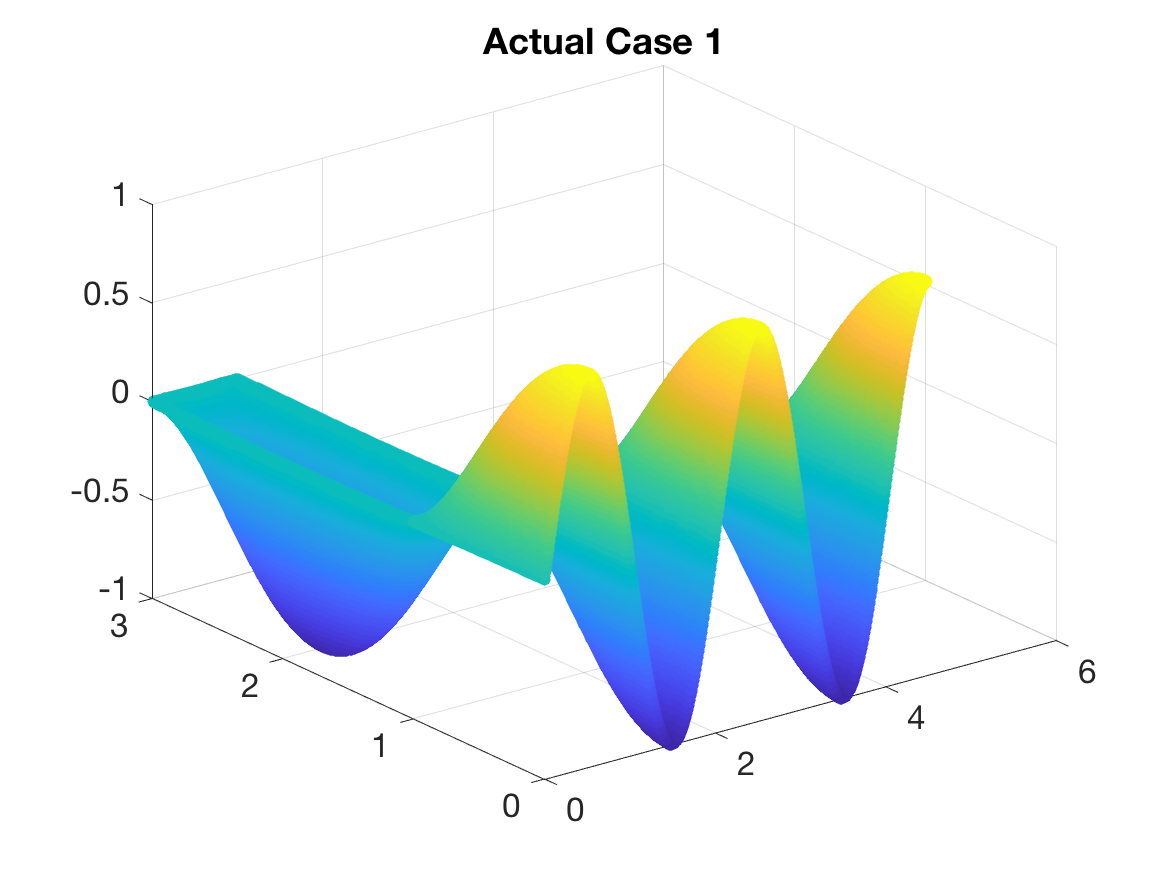
\includegraphics[width=0.3\linewidth]{../Figures/final_3_actual_1.png}&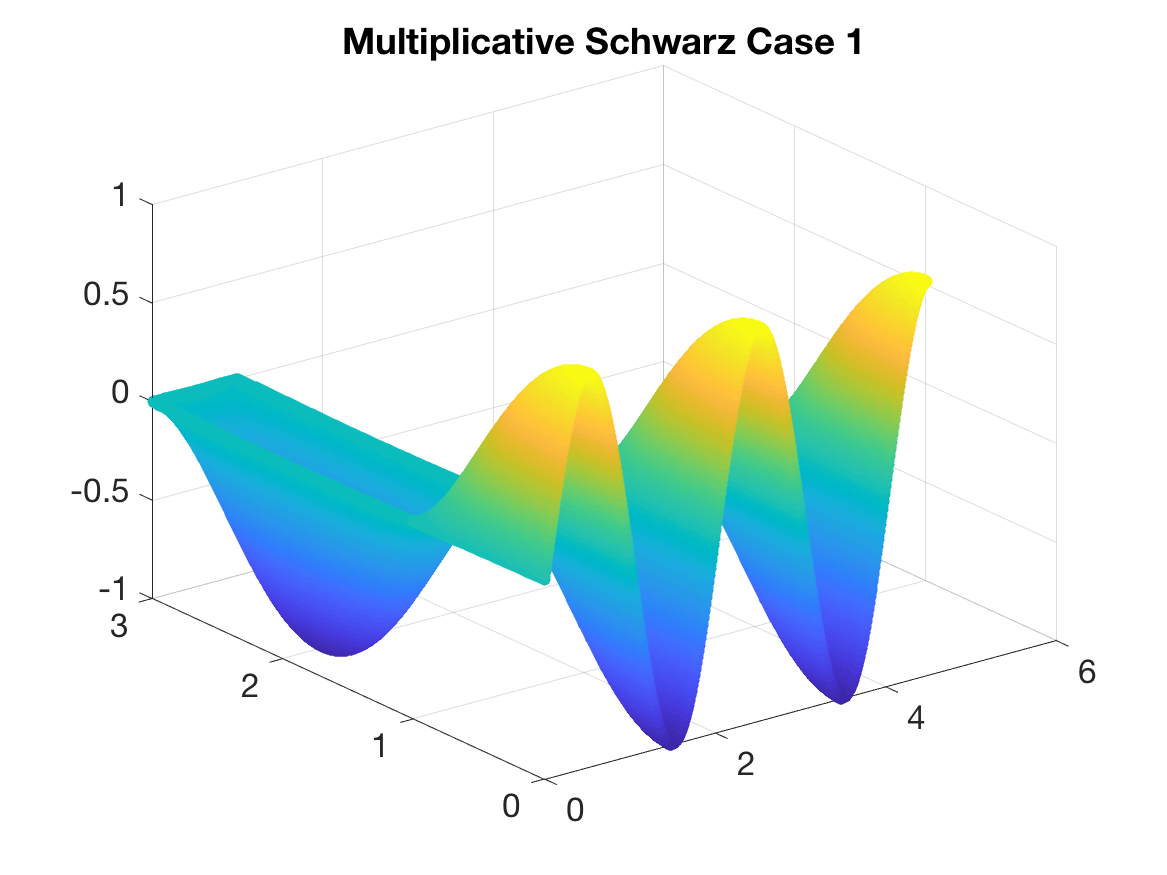
\includegraphics[width=0.3\linewidth]{../Figures/final_3_mult_1.png}&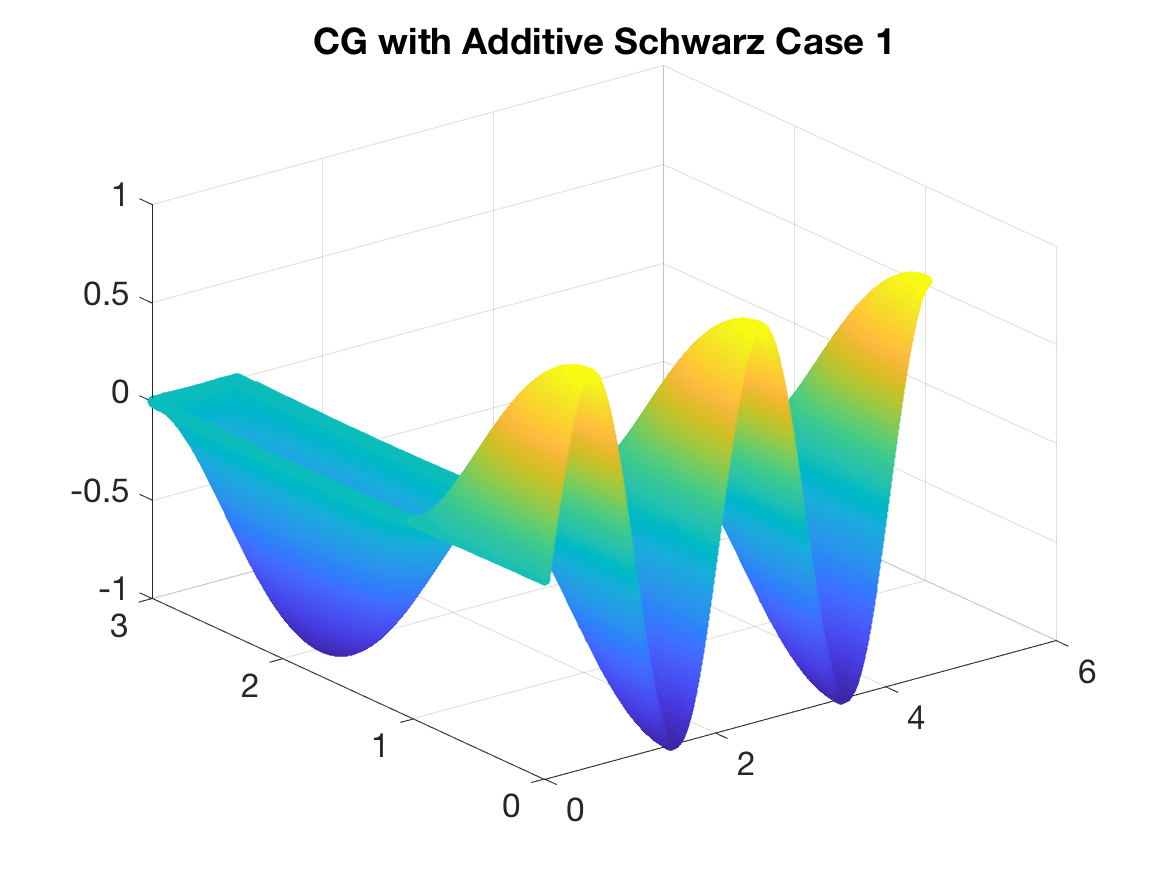
\includegraphics[width=0.3\linewidth]{../Figures/final_3_pcg_1.png}\\
    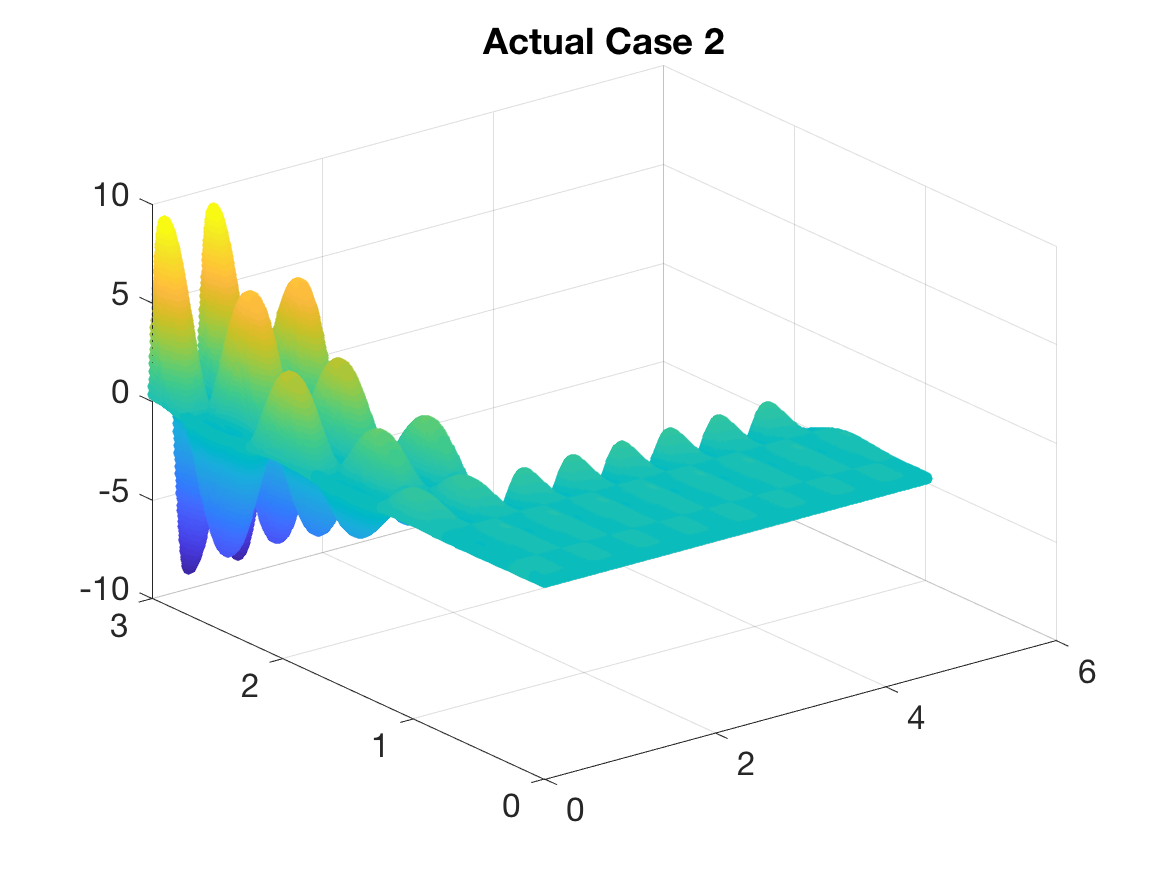
\includegraphics[width=0.3\linewidth]{../Figures/final_3_actual_2.png}&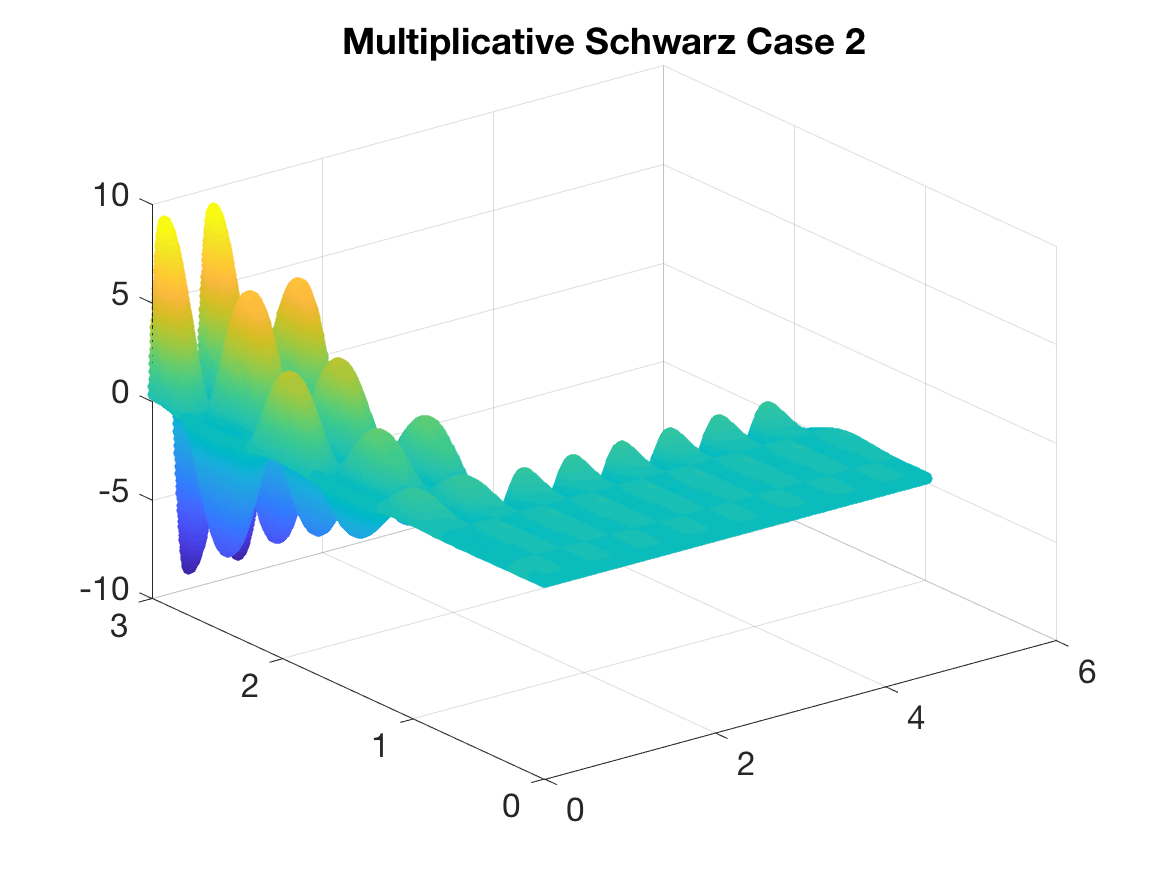
\includegraphics[width=0.3\linewidth]{../Figures/final_3_mult_2.png}&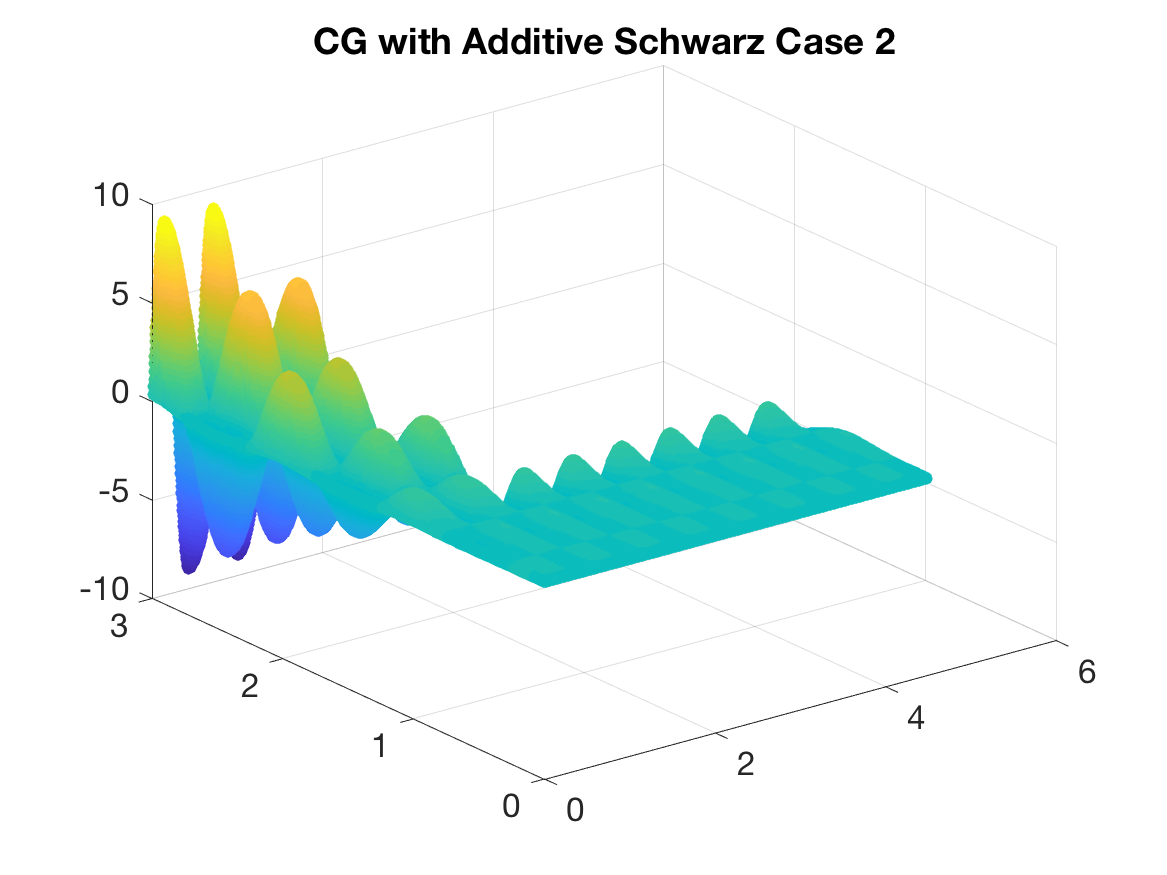
\includegraphics[width=0.3\linewidth]{../Figures/final_3_pcg_2.png}\\
    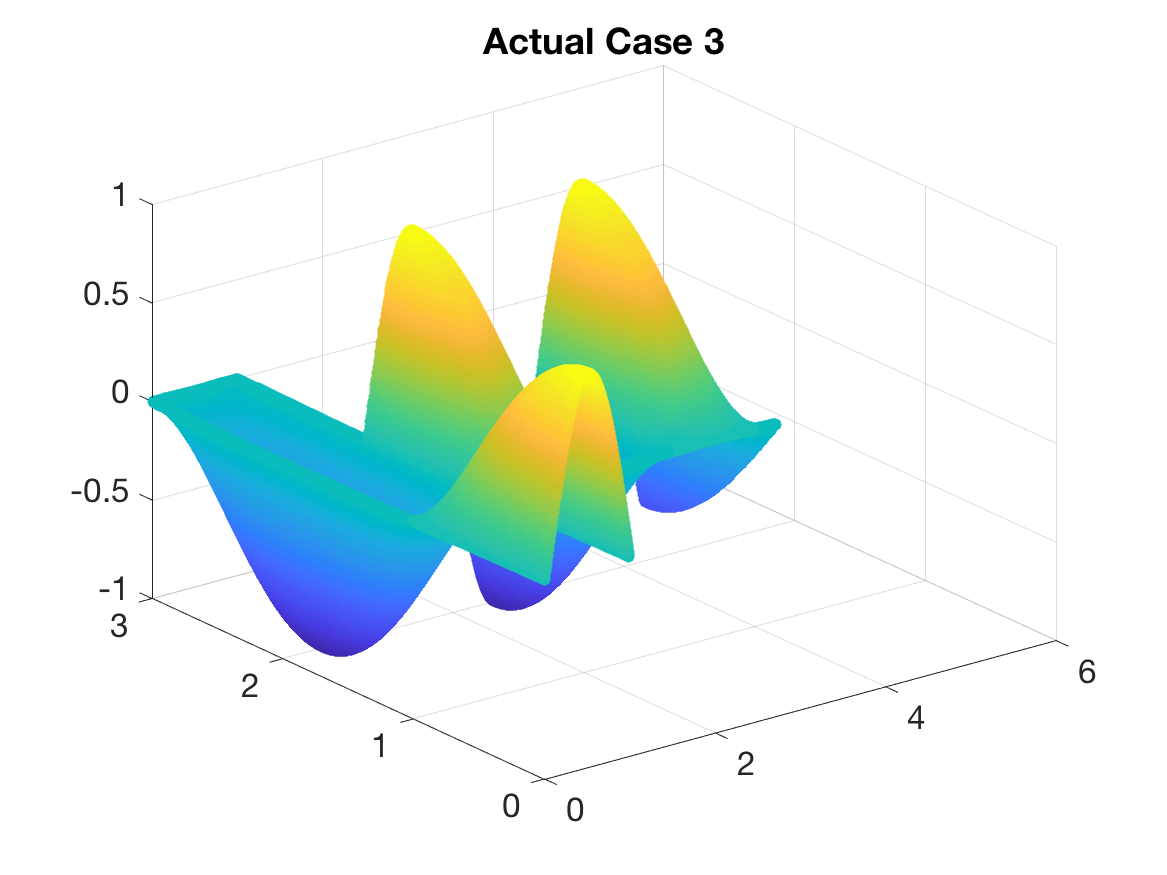
\includegraphics[width=0.3\linewidth]{../Figures/final_3_actual_3.png}&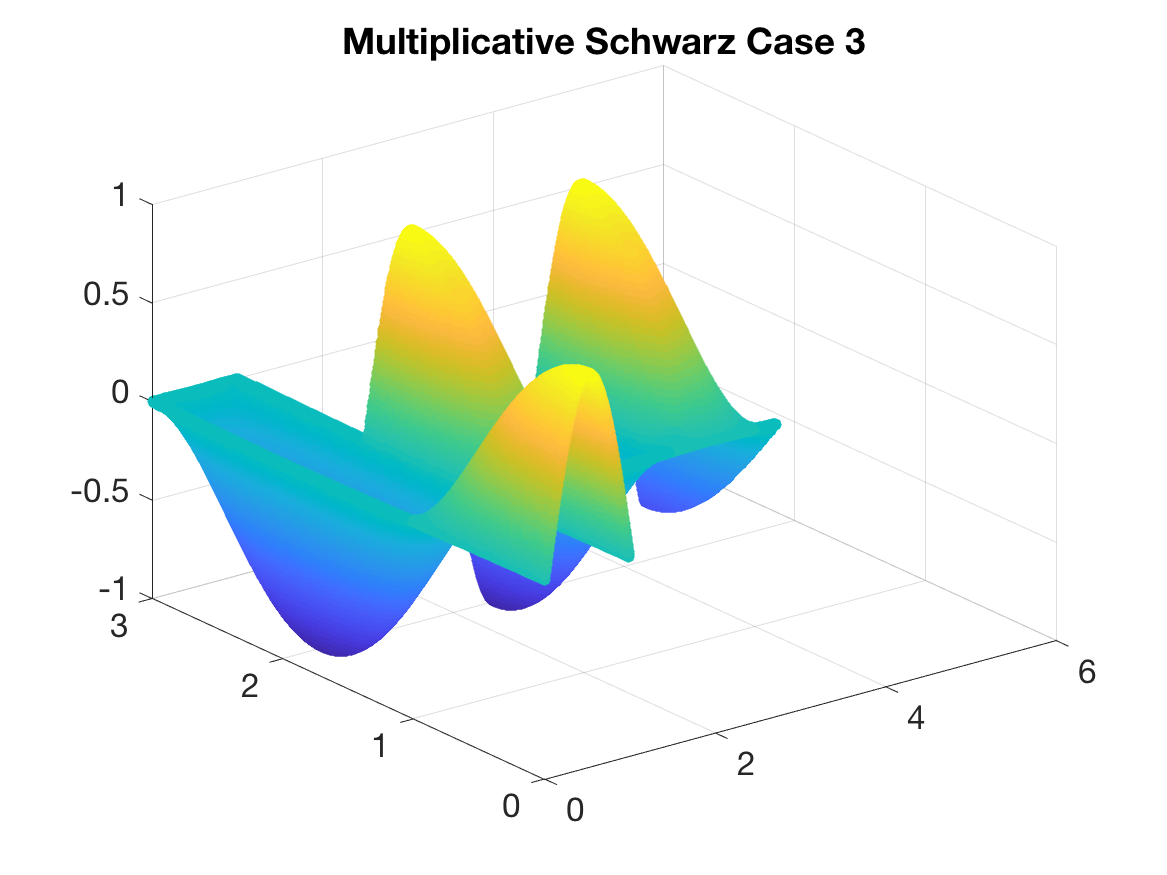
\includegraphics[width=0.3\linewidth]{../Figures/final_3_mult_3.png}&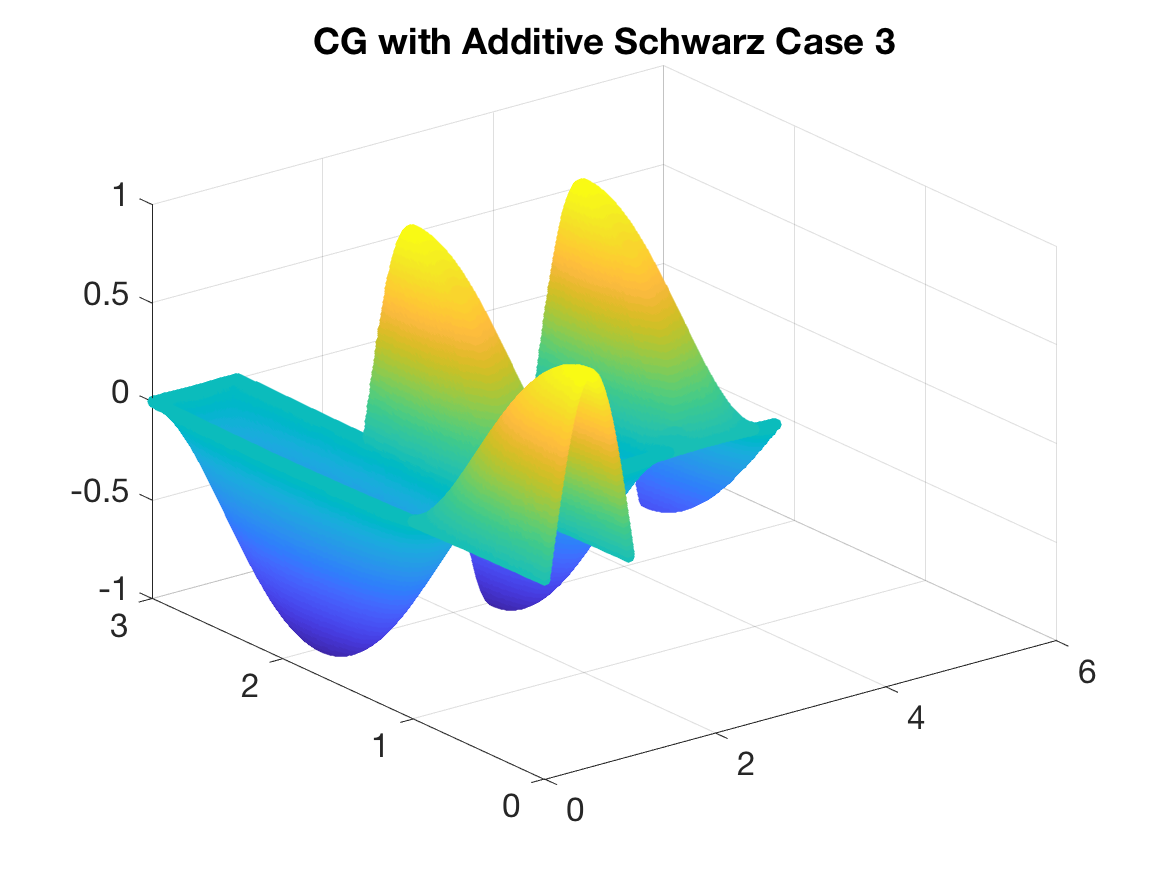
\includegraphics[width=0.3\linewidth]{../Figures/final_3_pcg_3.png}\\
    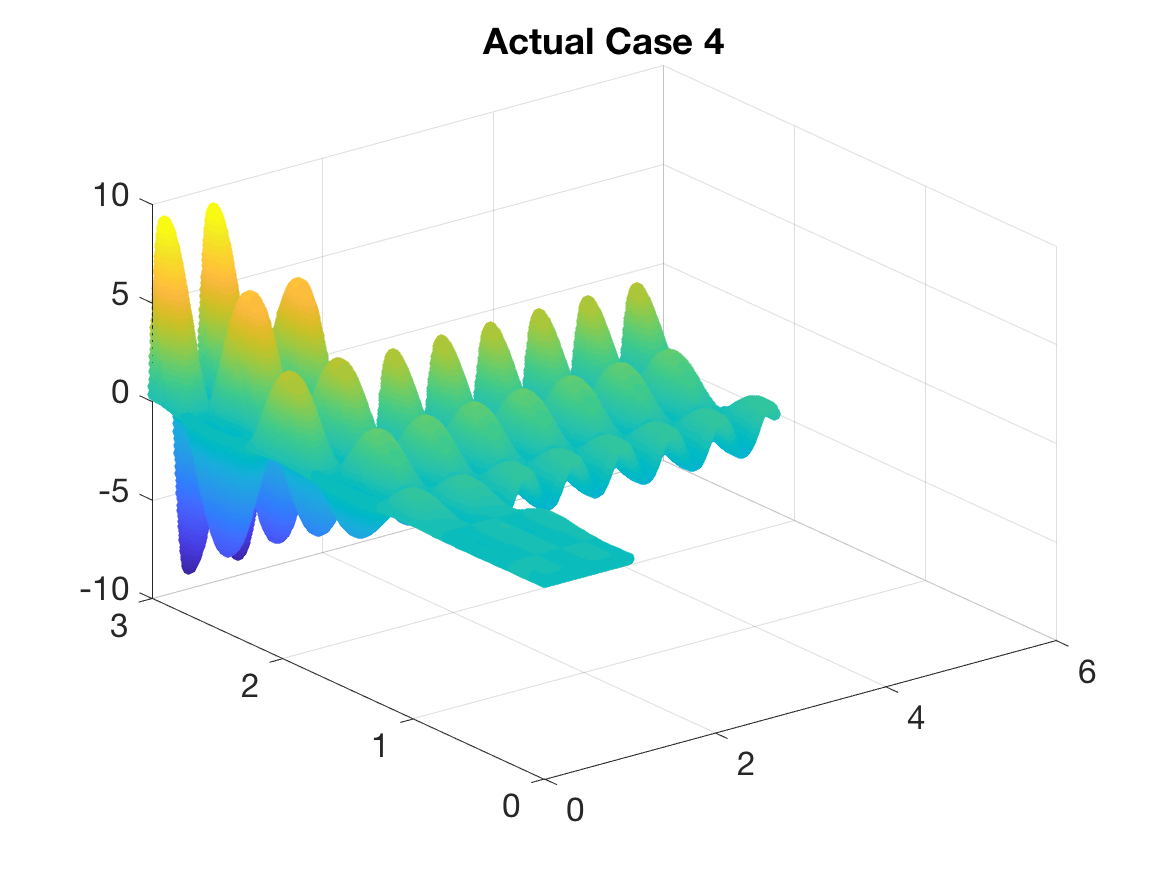
\includegraphics[width=0.3\linewidth]{../Figures/final_3_actual_4.png}&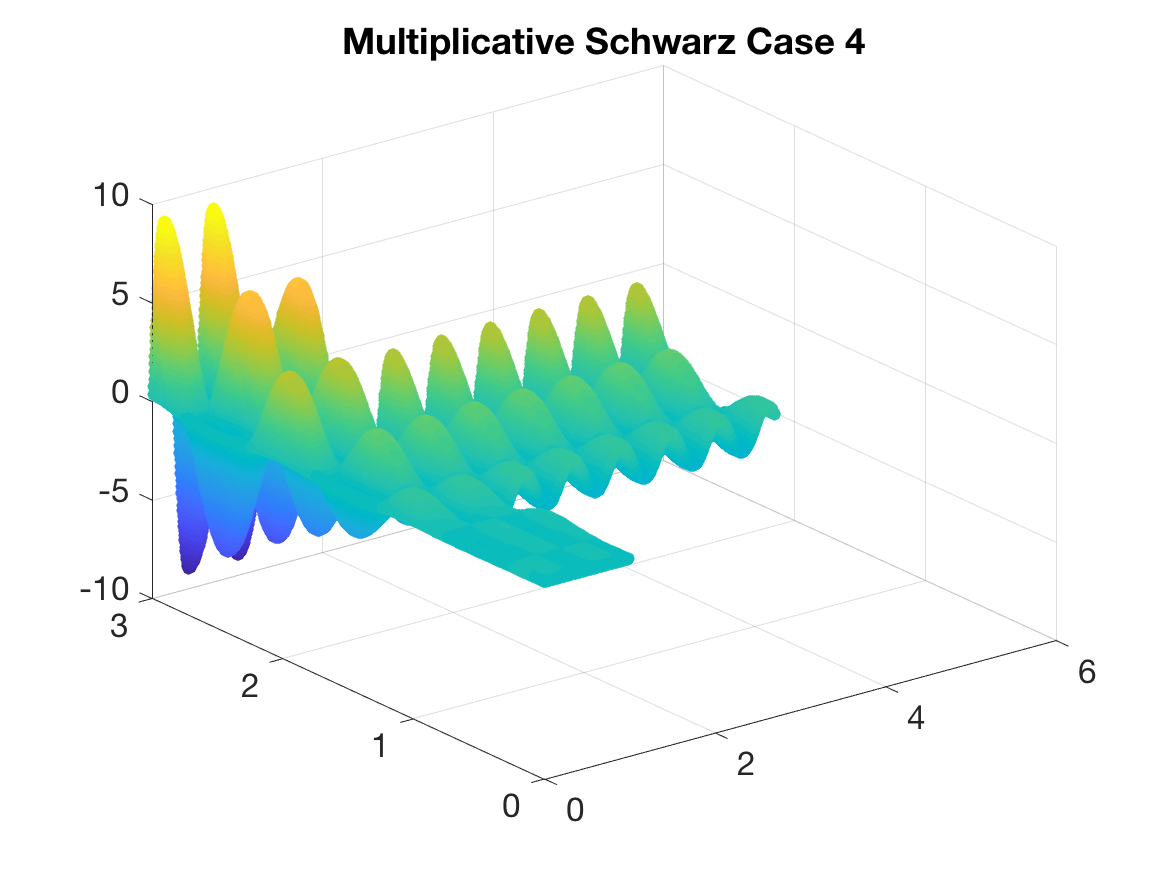
\includegraphics[width=0.3\linewidth]{../Figures/final_3_mult_4.png}&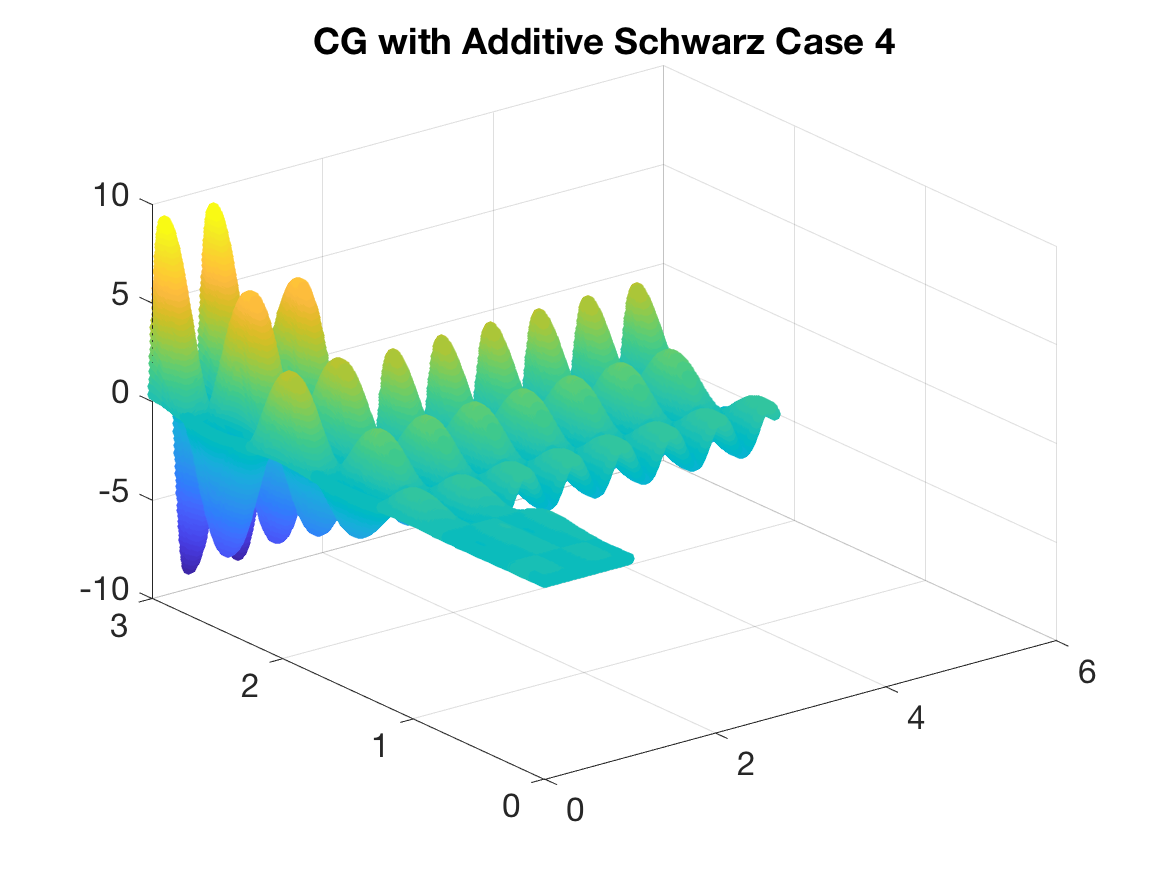
\includegraphics[width=0.3\linewidth]{../Figures/final_3_pcg_4.png}\\
    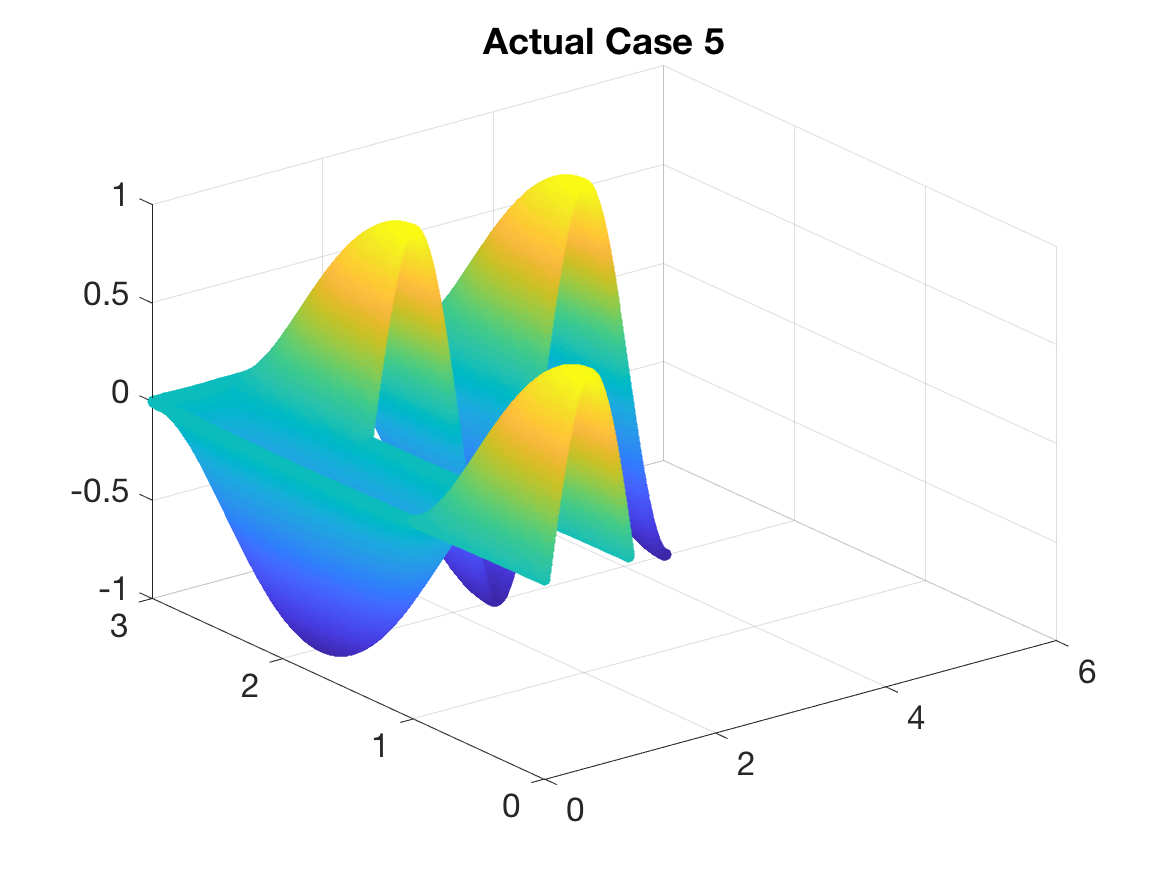
\includegraphics[width=0.3\linewidth]{../Figures/final_3_actual_5.png}&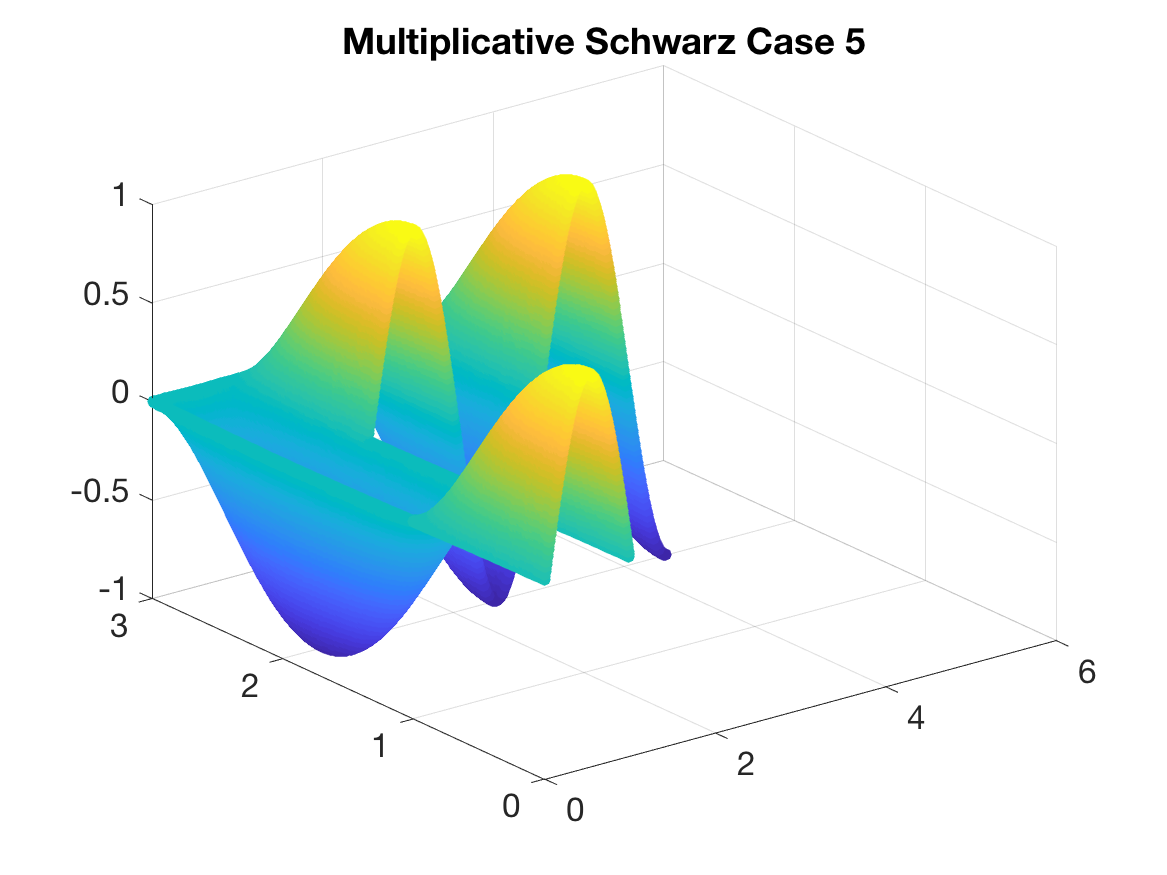
\includegraphics[width=0.3\linewidth]{../Figures/final_3_mult_5.png}&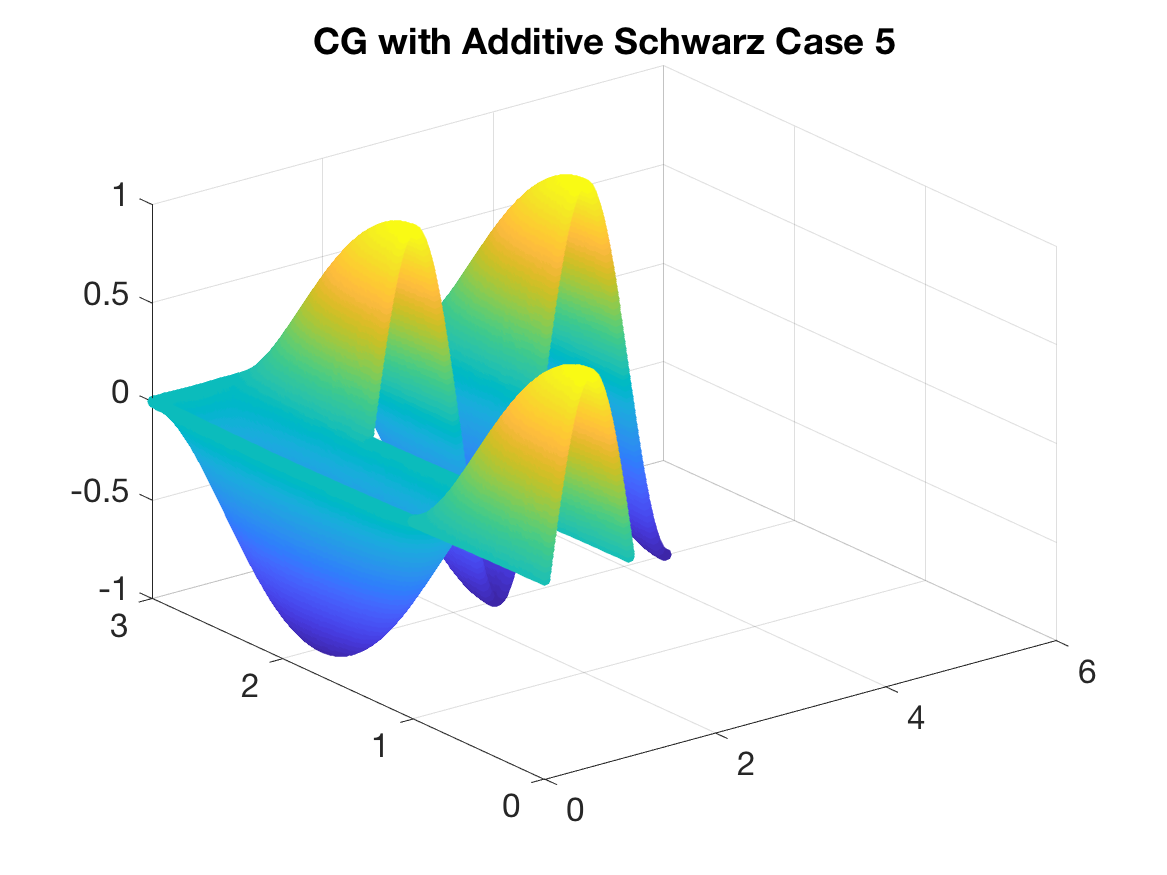
\includegraphics[width=0.3\linewidth]{../Figures/final_3_pcg_5.png}\\
    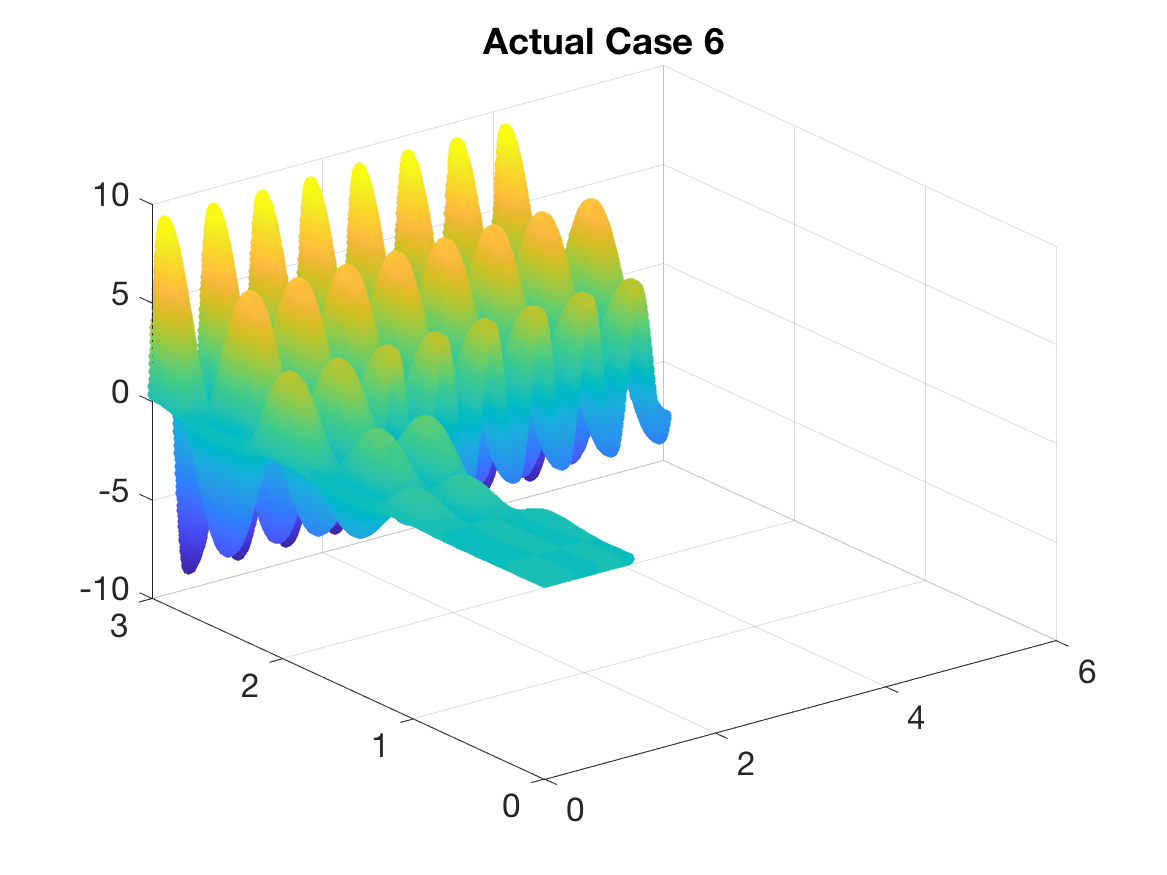
\includegraphics[width=0.3\linewidth]{../Figures/final_3_actual_6.png}&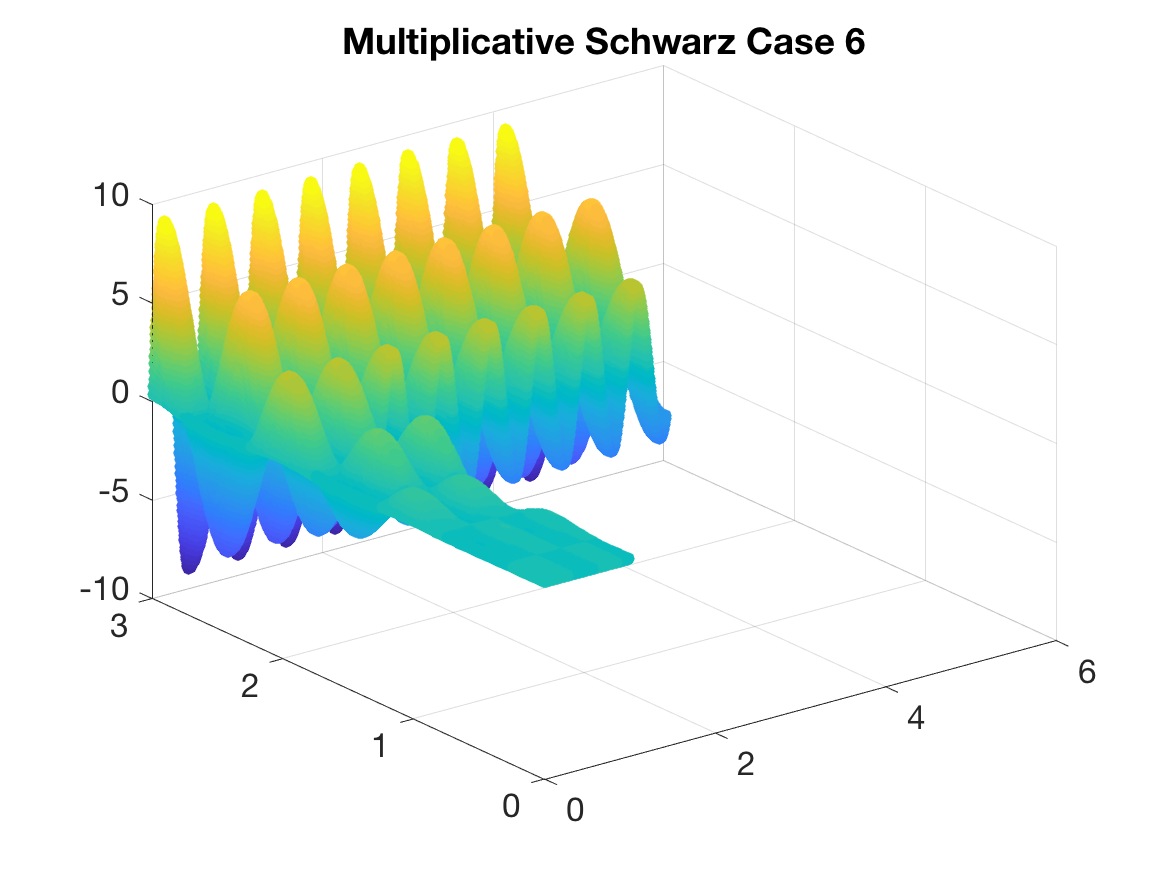
\includegraphics[width=0.3\linewidth]{../Figures/final_3_mult_6.png}&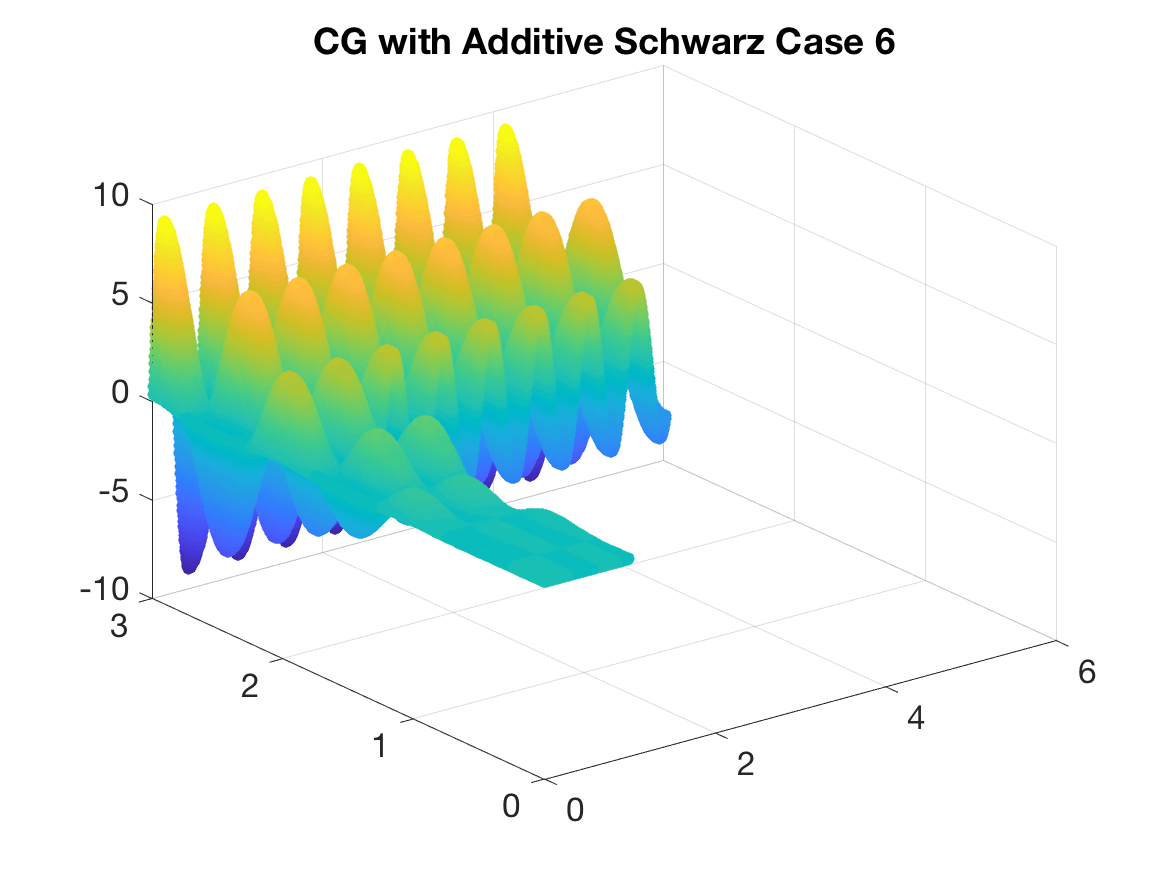
\includegraphics[width=0.3\linewidth]{../Figures/final_3_pcg_6.png}\\
  \end{tabular}
\end{center}

\newquestion
%======================================================
%
%                       Part 4
%
%======================================================
\section*{Part 4}

\lstinputlisting[style=Matlab-editor,basicstyle=\ttfamily\small]{../Code/alt_Schwarz.m}\newpage
\lstinputlisting[style=Matlab-editor,basicstyle=\ttfamily\small]{../Code/final_project_part_4.m}
\begin{center}
  \begin{tabular}{|c|c|c|c|c|}
    \hline
    &\multicolumn{2}{c|}{Discretized Alternating Schwarz}&\multicolumn{2}{c|}{GMRES with Preconditioner}\\\cline{2-5}
    Case&Relative Maximal Error&\# $R_1$ Solves& Relative Maximal Error &\# $R_1$ Solves\\\hline
    $\begin{array}{l}
       \textrm{(i)}\\
       \textrm{(ii)}\\
       \textrm{(iii)}\\
       \textrm{(iv)}\\
       \textrm{(v)}\\
       \textrm{(vi)}
     \end{array}$&$\begin{array}{r}
\texttt{8.826018913059459e-04}\\
\texttt{2.204336957196286e-03}\\
\texttt{8.859326481153902e-04}\\
\texttt{2.101333790306490e-02}\\
\texttt{6.033999160146575e-04}\\
\texttt{1.636715246570604e-02}\\
\end{array}
$&$\begin{array}{r}
\texttt{30}\\
\texttt{30}\\
\texttt{30}\\
\texttt{30}\\
\texttt{30}\\
\texttt{30}\\
\end{array}
$&$\begin{array}{r}
\texttt{0.000000000000000e+00}\\
\end{array}
$&$\begin{array}{r}
\texttt{0}\\
\end{array}
$\\\hline
  \end{tabular}
\end{center}

\begin{center}
  \begin{tabular}{ccc}
    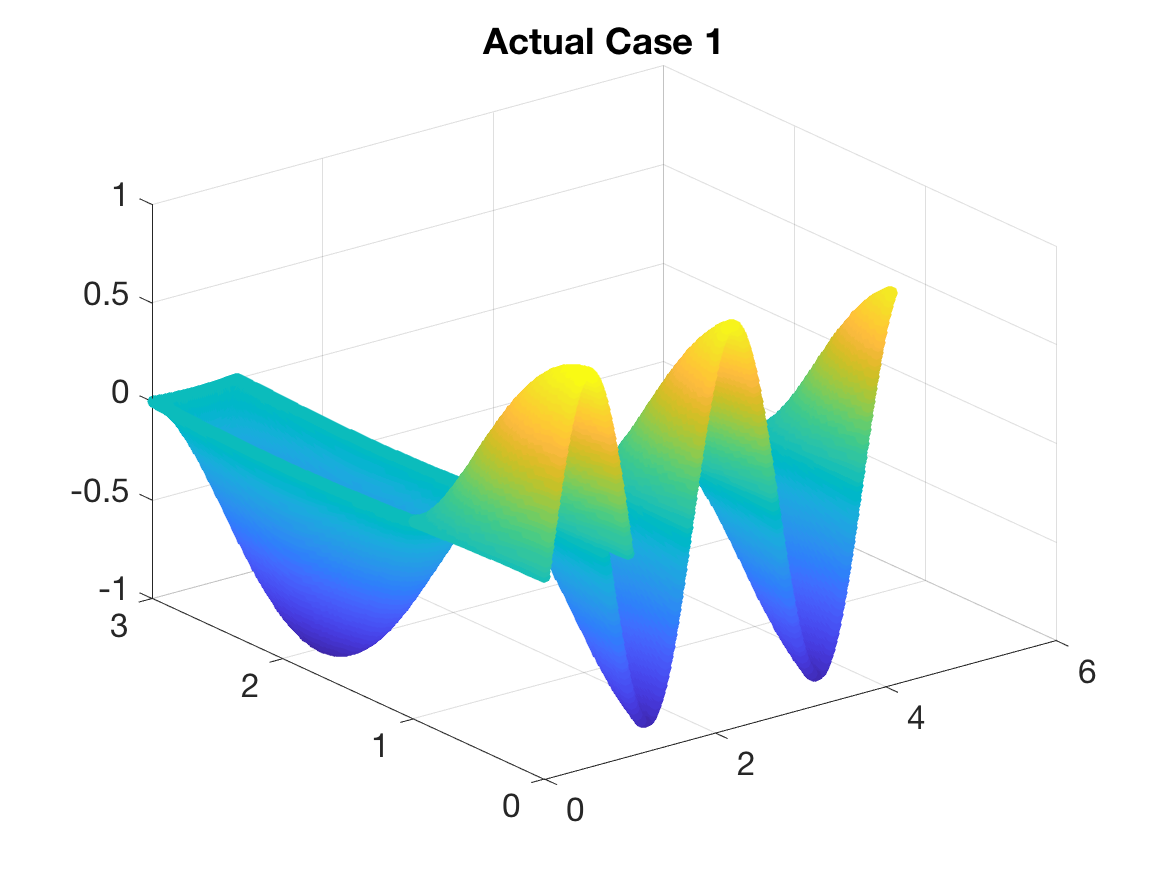
\includegraphics[width=0.3\linewidth]{../Figures/final_4_actual_1.png}&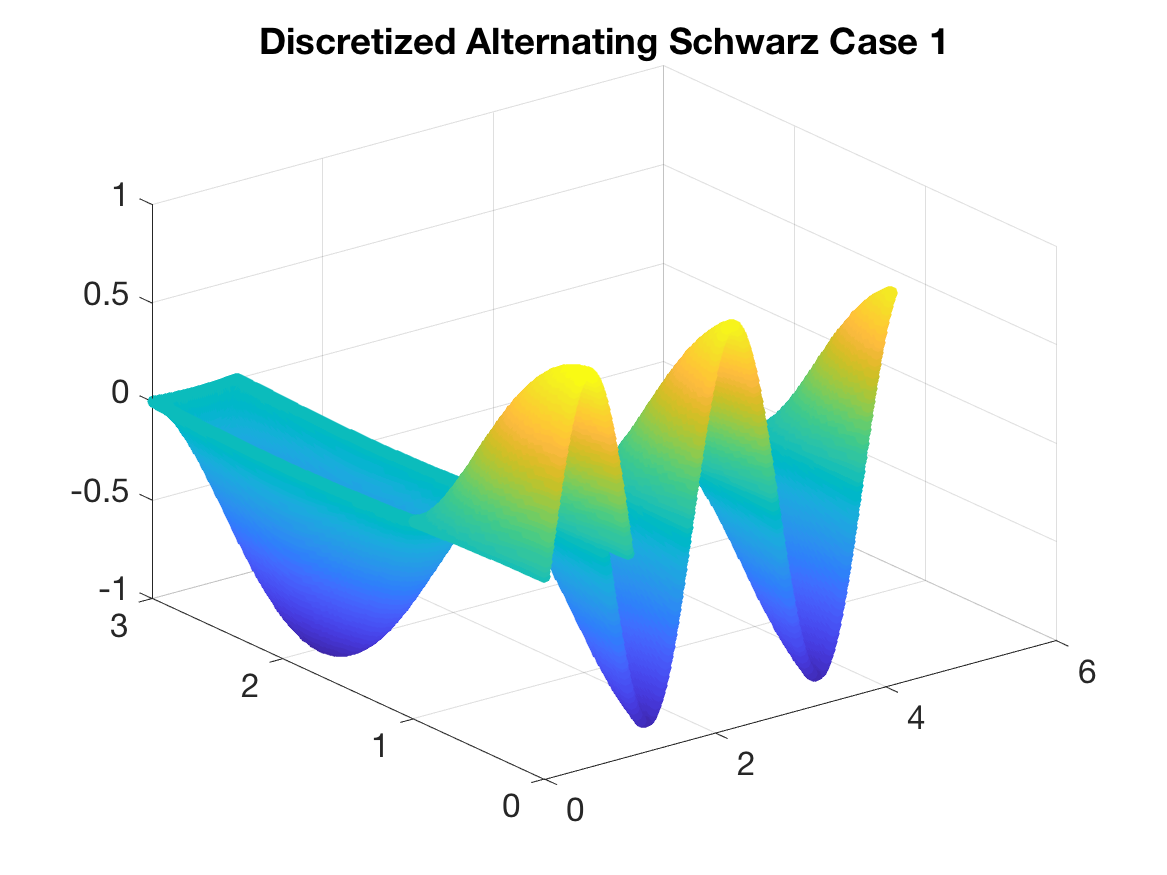
\includegraphics[width=0.3\linewidth]{../Figures/final_4_add_1.png}&\\
    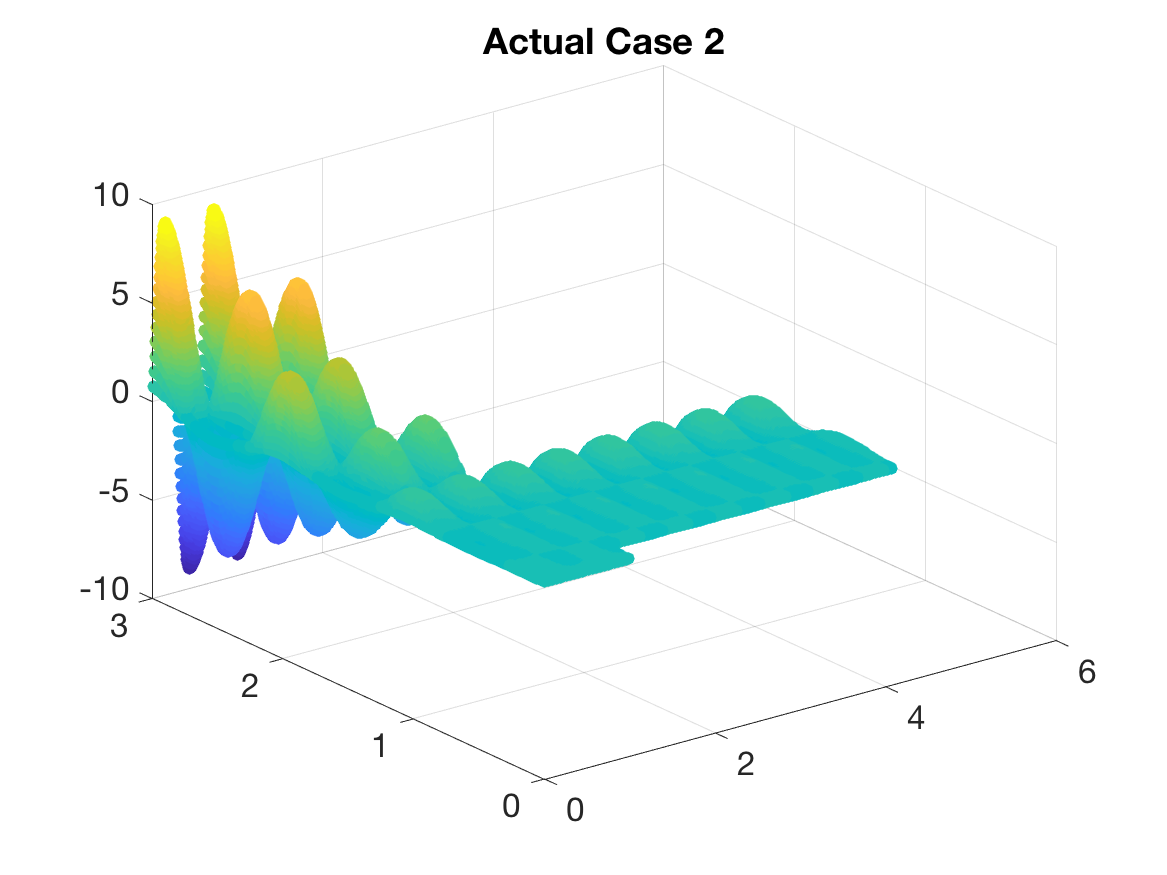
\includegraphics[width=0.3\linewidth]{../Figures/final_4_actual_2.png}&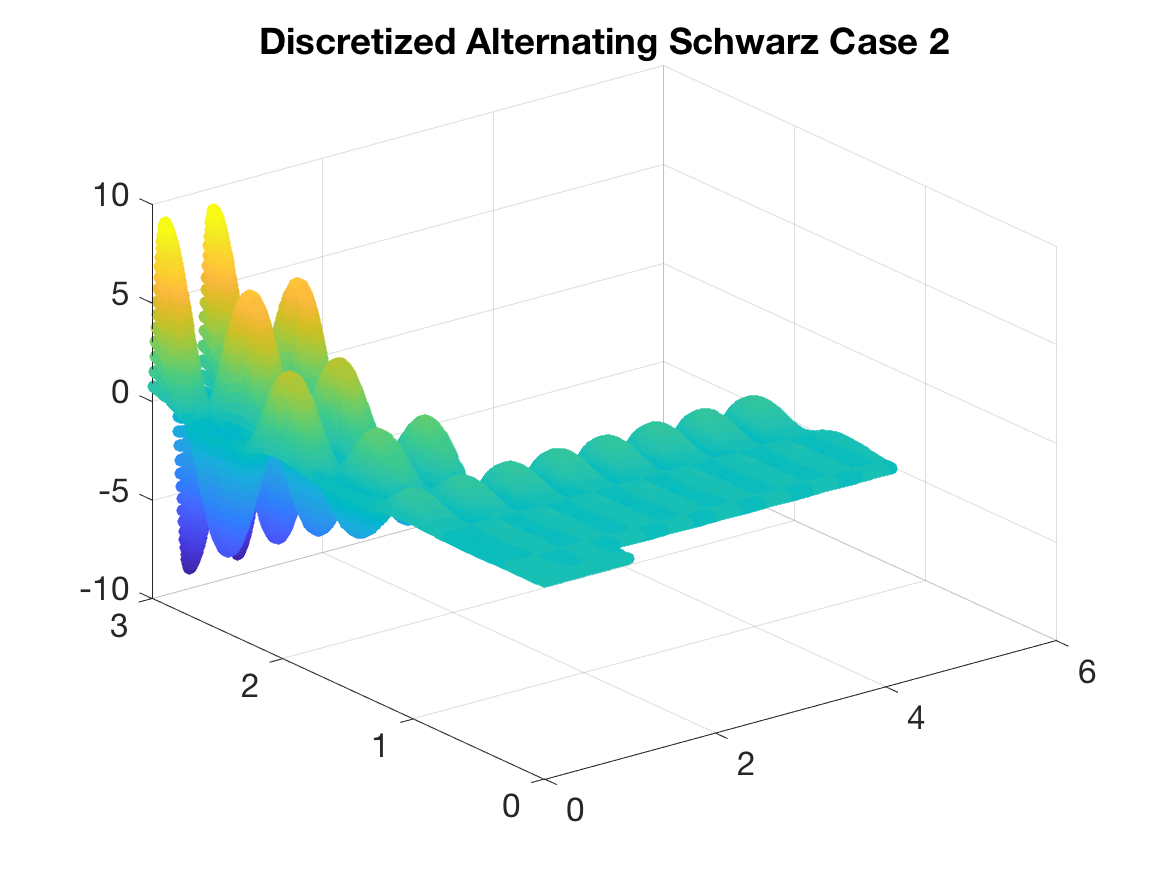
\includegraphics[width=0.3\linewidth]{../Figures/final_4_add_2.png}&\\
    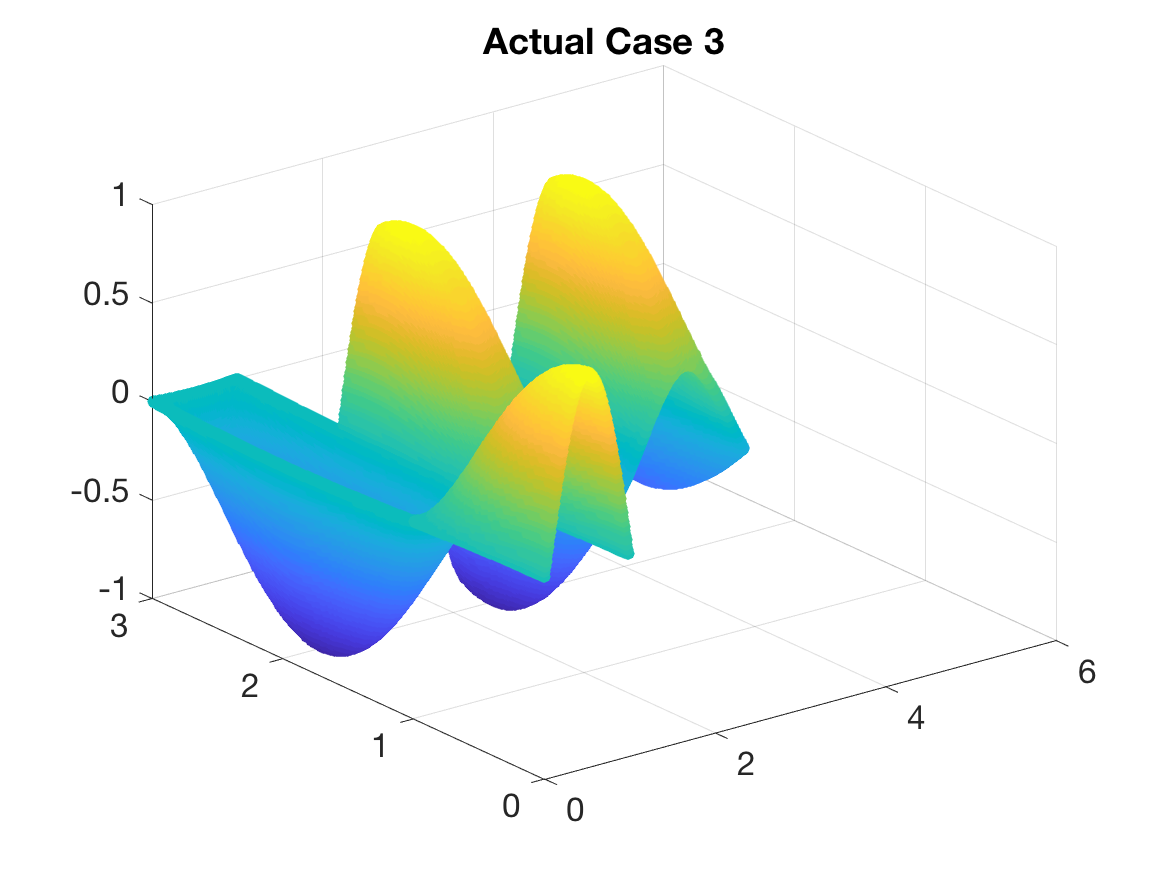
\includegraphics[width=0.3\linewidth]{../Figures/final_4_actual_3.png}&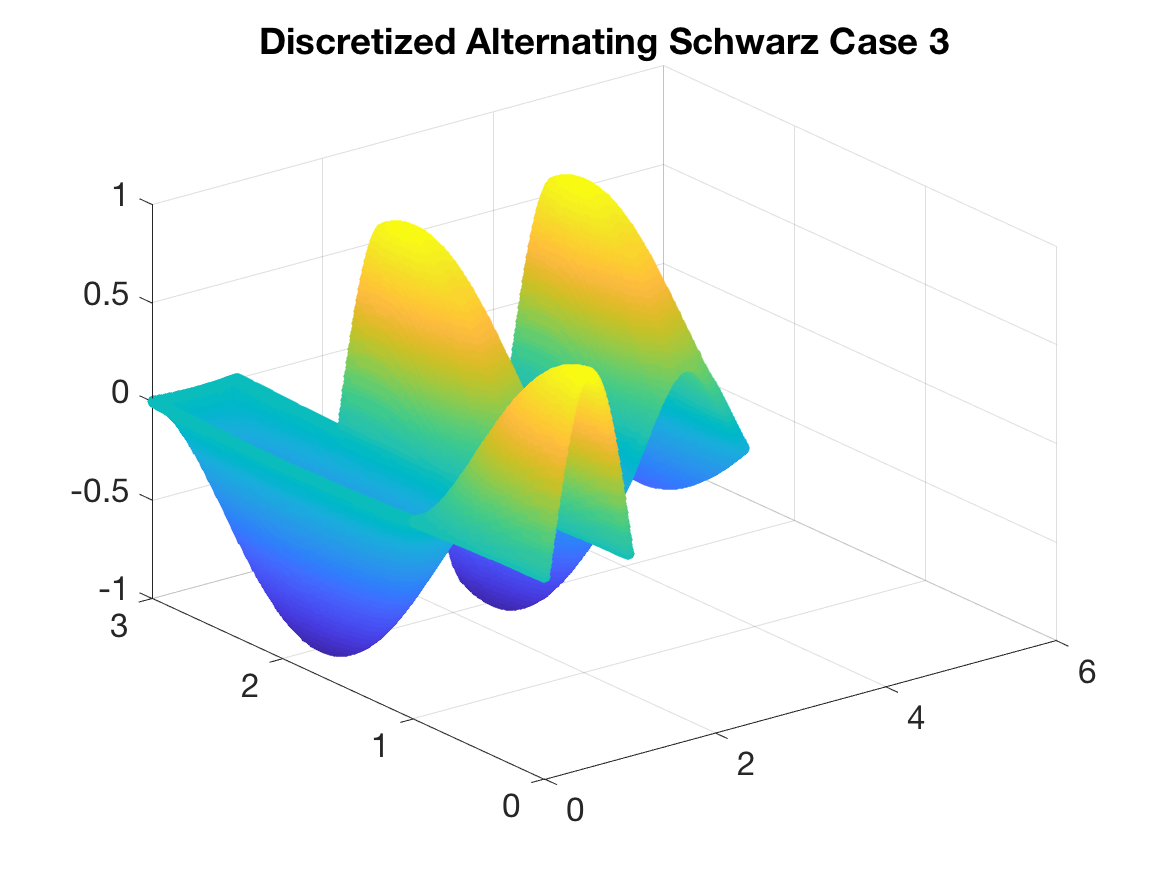
\includegraphics[width=0.3\linewidth]{../Figures/final_4_add_3.png}&\\
    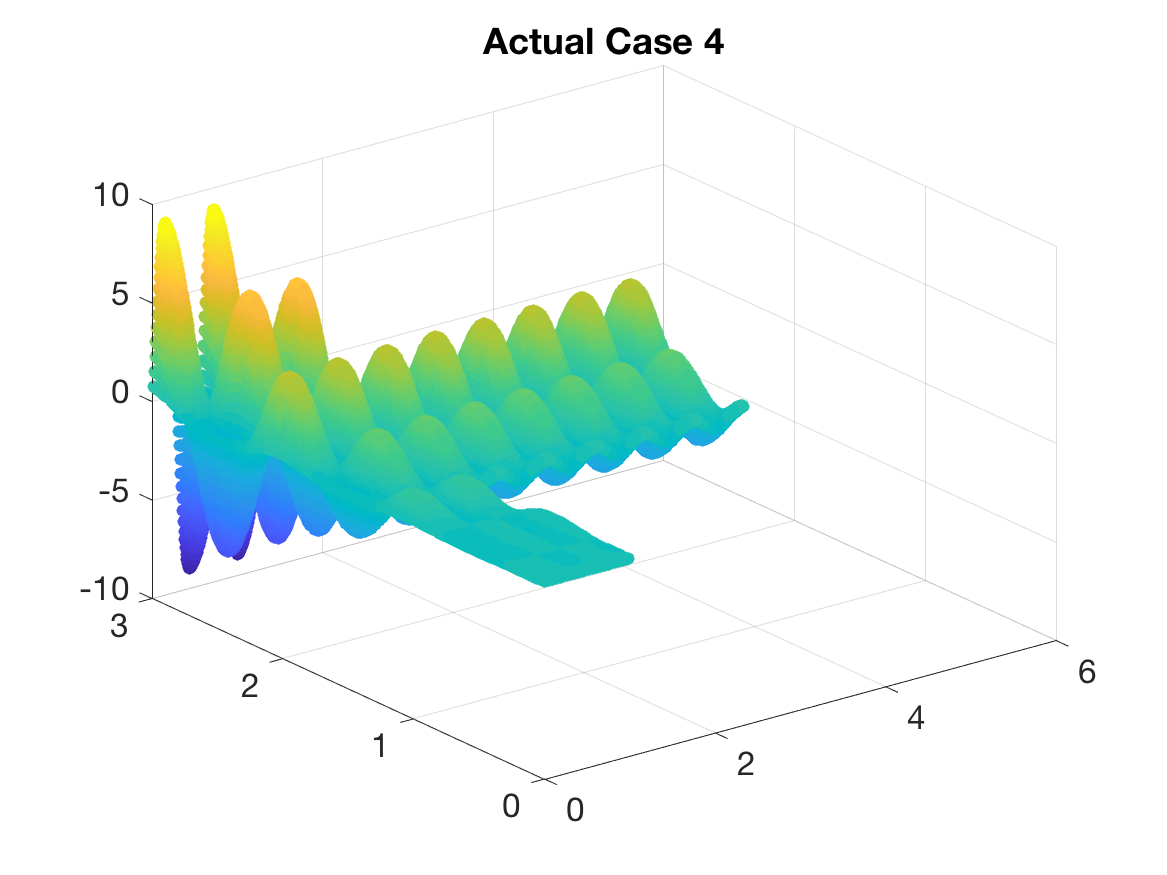
\includegraphics[width=0.3\linewidth]{../Figures/final_4_actual_4.png}&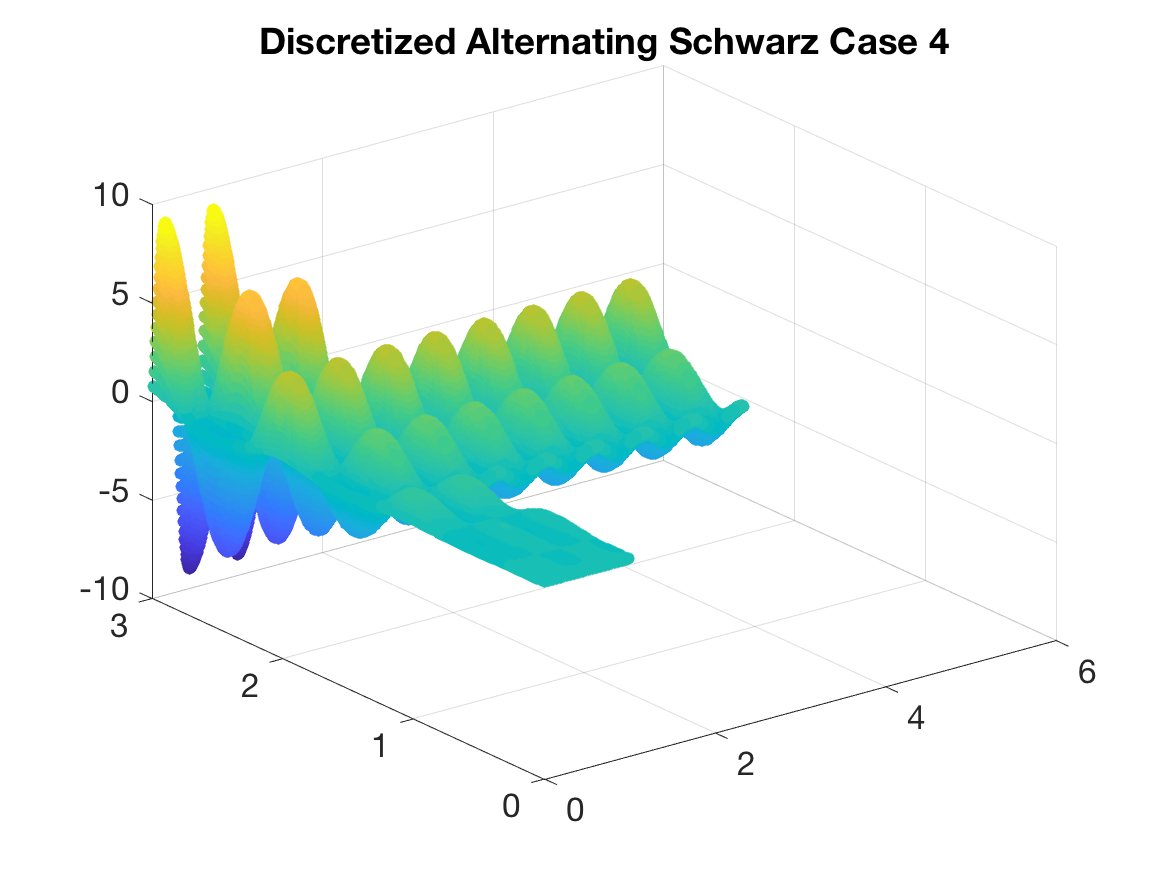
\includegraphics[width=0.3\linewidth]{../Figures/final_4_add_4.png}&\\
    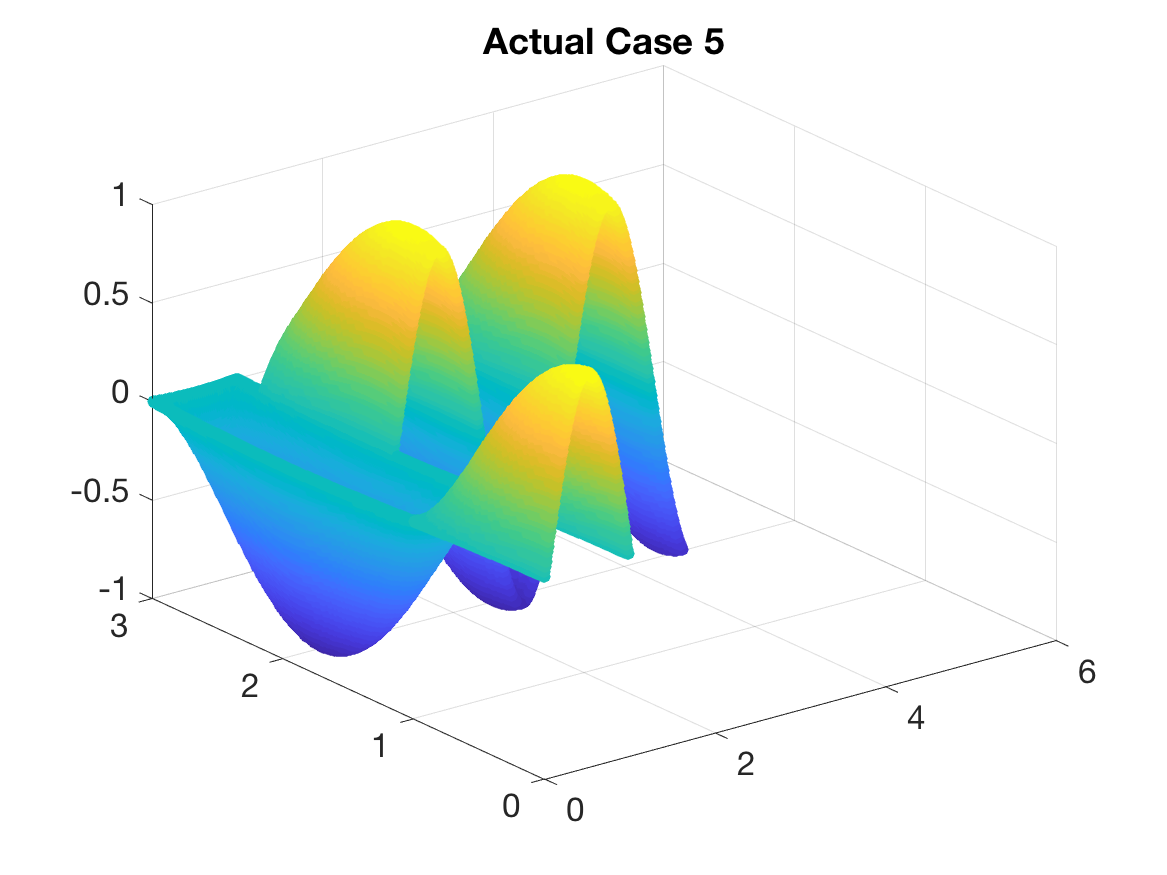
\includegraphics[width=0.3\linewidth]{../Figures/final_4_actual_5.png}&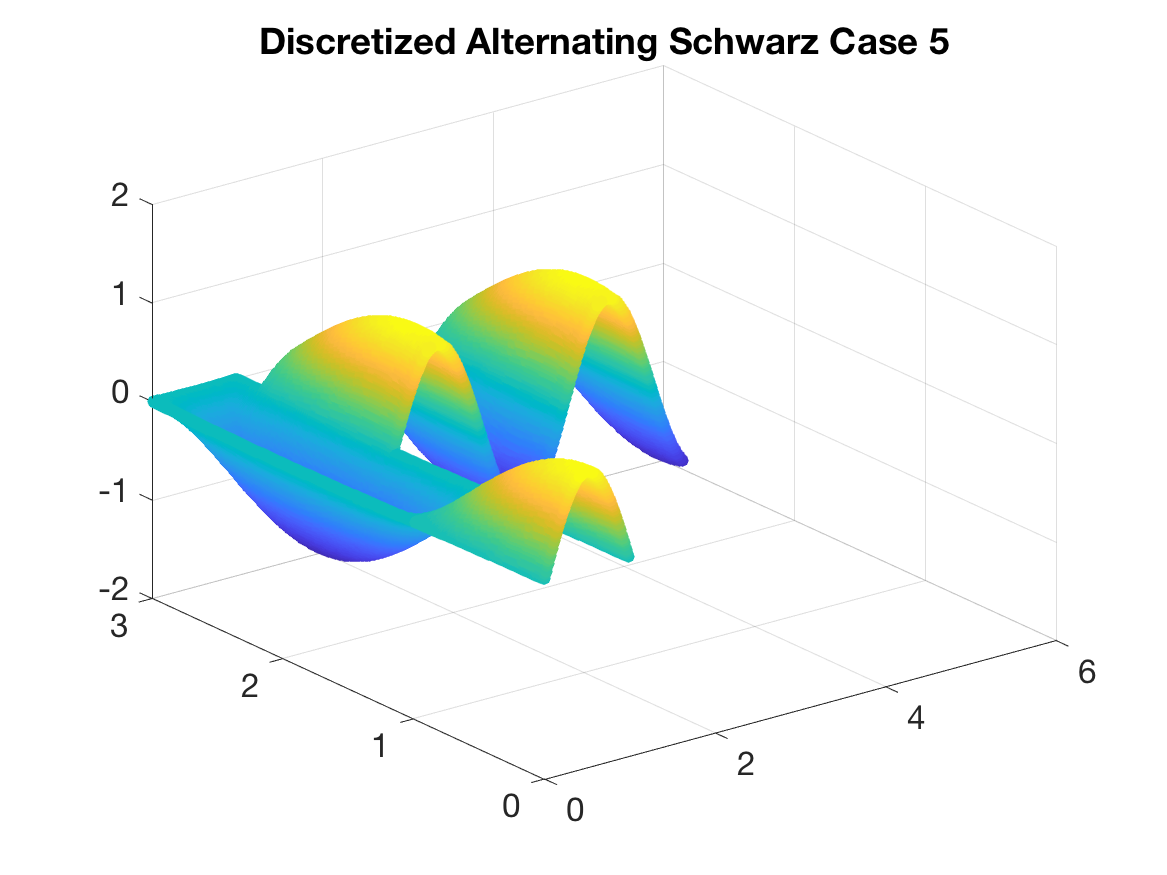
\includegraphics[width=0.3\linewidth]{../Figures/final_4_add_5.png}&\\
    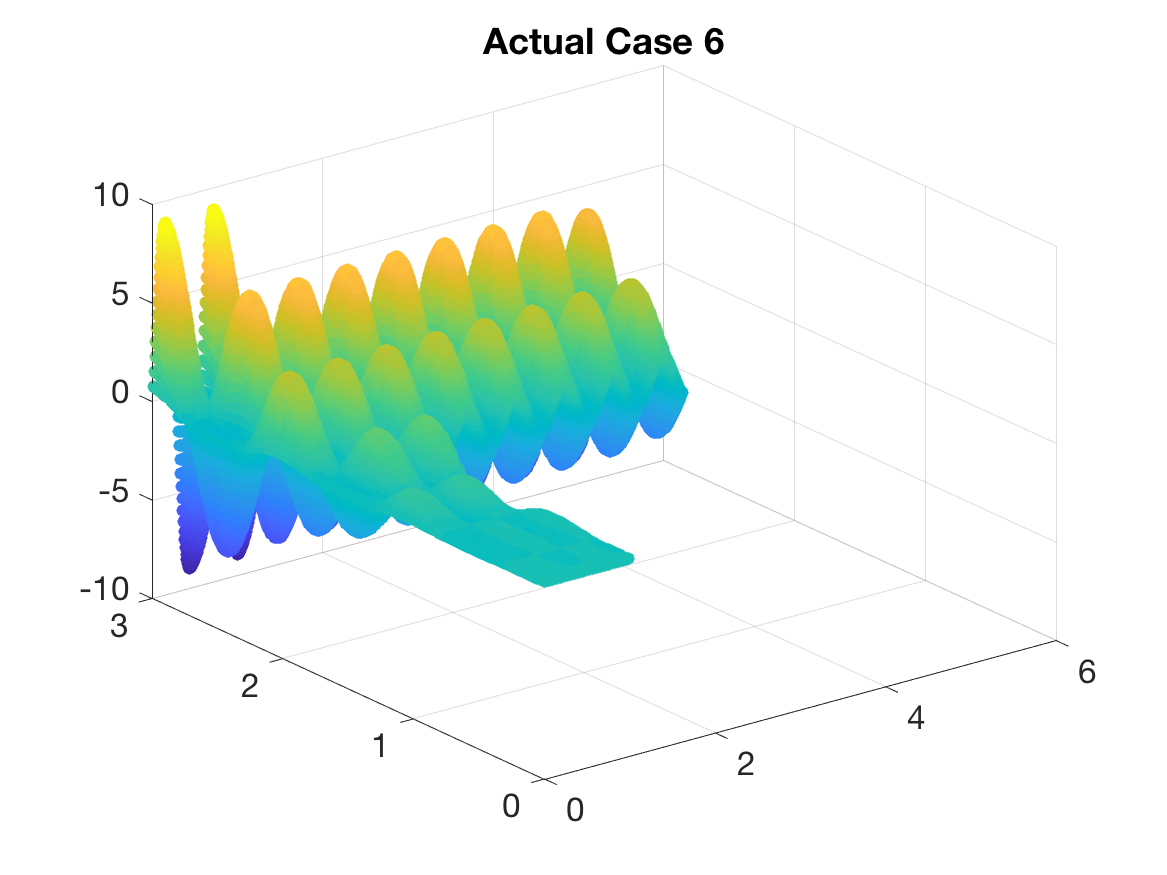
\includegraphics[width=0.3\linewidth]{../Figures/final_4_actual_6.png}&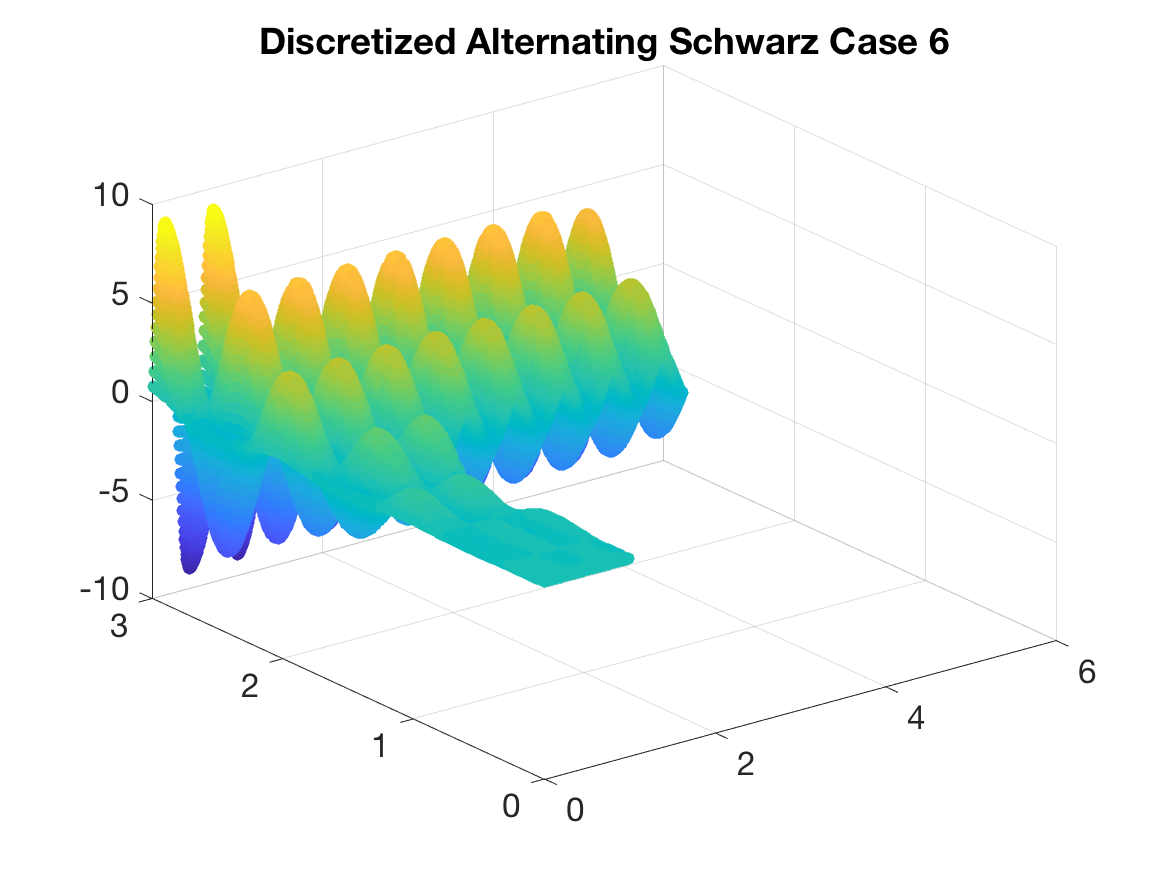
\includegraphics[width=0.3\linewidth]{../Figures/final_4_add_6.png}&
  \end{tabular}
\end{center}

\end{document}
%================================================================
%================================================================
%
%                           Templates
%
%================================================================
%================================================================


%----------------------------------------------------------------
%----------------------------------------------------------------

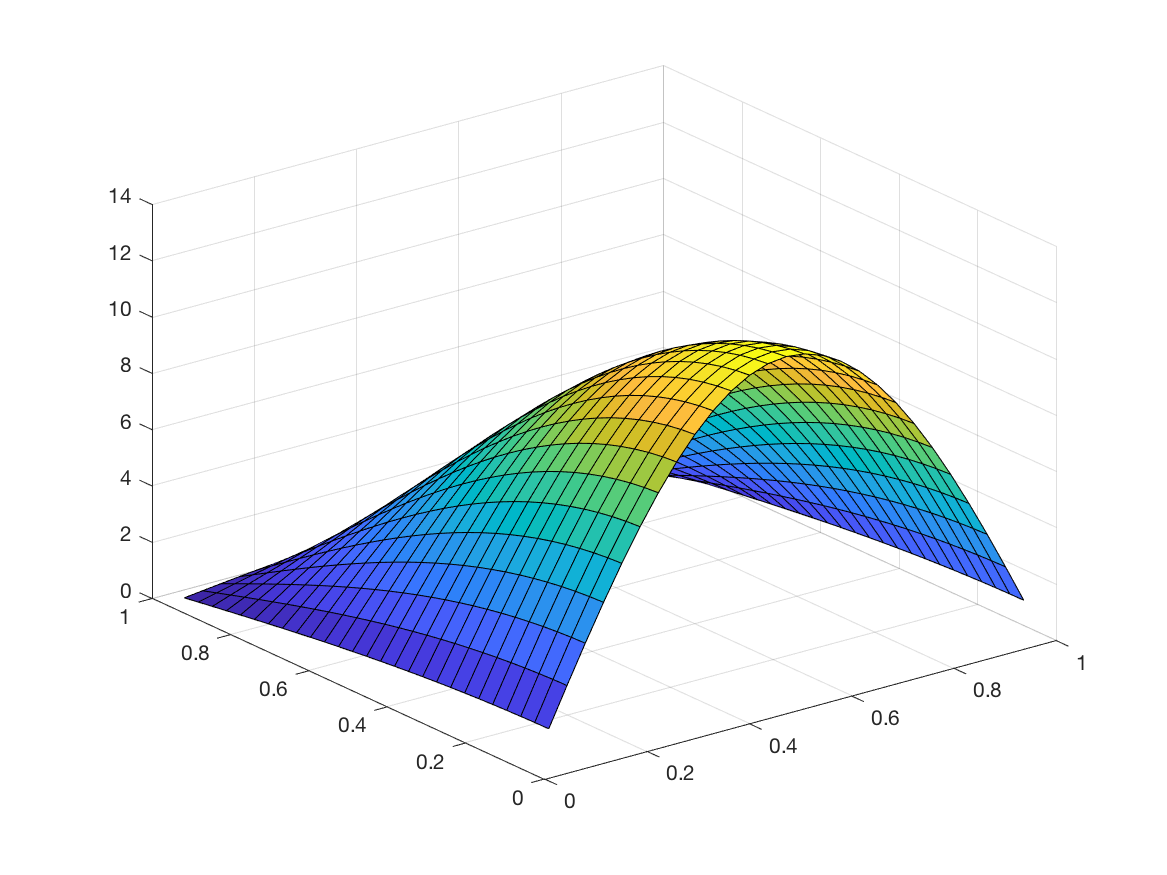
\includegraphics[width=\linewidth]{../Figures/poisson_rhs_1.png}
\lstinputlisting[style=Matlab-editor,basicstyle=\ttfamily\small]{../Code/solvePoisson.m}

\newquestion
%======================================================
%
%                    Problem n
%
%======================================================
\section*{Problem n}

\newpart
%--------------------------
%    Problem n Part A
%--------------------------
\subsection*{(a)}

\newpart
%--------------------------
%    Problem n Part B
%--------------------------
\subsection*{(b)}


%----------------------------------------------------------------
%----------------------------------------------------------------


%======================================================
%
%               Appendix: Problem n
%
%======================================================
%--------------------------
%  Appendix: P n Part A
%--------------------------
\subsection*{Problem n Part A}

\newpage
%--------------------------
%  Appendix: P n Part B
%--------------------------
\subsection*{Problem n Part B}


%----------------------------------------------------------------
%----------------------------------------------------------------


The centered-difference approximation for the partial difference equations has the form:
\begin{eqnarray*}
  h^{-2}\left(2v_{j,k}-v_{j-1,k}-v_{j+1,k}\right)+h^{-2}\left(2v_{j,k}-v_{j,k-1}-v_{j,k+1}\right)&=&f\left(x_j,y_k\right)\\
  h^{-2}T_{m_x}V+h^{-2}VT_{m_y}-h^{-2}B-h^{-2}C&=&F\\
  T_{m_x}V+VT_{m_y}&=&h^2F+B+C
\end{eqnarray*}
where
\begin{align*}
  B&=\left[
  \begin{array}{cccc}
    b_{01}&b_{02}&\cdots&b_{0m}\\
    0&0&\cdots&0\\
    \vdots&\vdots&&\vdots\\
    0&0&\cdots&0\\
    b_{11}&b_{12}&\cdots&b_{1m}\\
  \end{array}
  \right]\qquad &C&=\left[
  \begin{array}{ccccc}
    c_{01}&0&\cdots&0&c_{11}\\
    c_{02}&0&\cdots&0&c_{12}\\
    \vdots&\vdots&&\vdots&\vdots\\
    c_{0m}&0&\cdots&0&c_{1m}\\
  \end{array}
  \right]\\
  b_{0j}&=g\left(x_j,0\right)&c_{0k}&=g\left(0,y_k\right)\\
  b_{1j}&=g\left(x_j,b\right)&c_{1k}&=g\left(a,y_k\right)\\
  x_j&=jh&y_k&=khh&=\frac{1}{2^m}
\end{align*}
and thus
\begin{eqnarray*}
  Z_{m_x}^TT_{m_x}Z_{m_x}Z_{m_x}^TVZ_{m_y}+Z_{m_x}^TVZ_{m_y}Z_{m_y}^TVZ_{m_y}&=&Z_{m_x}^T\tilde{F}Z_{m_y}^T\\
  \Lambda_{m_x} V'+V'\Lambda_{m_y}&=&\tilde{F}'\\
  \lambda_j v_{jk}'+v_{jk}'\lambda_k&=&\tilde{f}_{jk}'\\
  v_{jk}'&=&\frac{\tilde{f_{jk}}'}{\lambda_{j}+\lambda_k}\\
  V&=&Z_{m_x}^TV'Z_{m_y}
\end{eqnarray*}
where
\begin{align*}
  \lambda_j&=2\left(1-\cos\left(\frac{\pi hj}{b-a}\right)\right)&\lambda_k&=2\left(1-\cos\left(\frac{\pi hk}{d-c}\right)\right)
\end{align*}\newpage